% \documentclass{article}
\documentclass[journal]{IEEEtran}
\usepackage[utf8]{inputenc}
\usepackage{amsmath}

%%%%% ADDED BY TOMMY %%%%%
\usepackage{xcolor}
\usepackage{xspace}
\usepackage{amsfonts}
\usepackage{graphicx}
\usepackage{booktabs}
\usepackage{hyperref}
\usepackage{authblk}
\usepackage{hyperref}
\usepackage{placeins}
% \usepackage{subfigure}
 
\DeclareMathOperator*{\argmin}{arg\,min}
\DeclareMathOperator*{\argmax}{arg\,max}
\newtheorem{definition}{Definition}
\newtheorem{lemma}{Lemma}
\newcommand{\Ie}{\textit{I.e.}\xspace}
\newcommand{\ie}{\textit{i.e.}\xspace}
\newcommand{\Eg}{\textit{E.g.}\xspace}
\newcommand{\eg}{\textit{e.g.}\xspace}
\newcommand{\probP}{\text{I\kern-0.15em P}}

\DeclareMathOperator*{\minimise}{\textrm{minimise}}
\DeclareMathOperator*{\maximise}{\textrm{maximise}}

\newcommand{\tl}[1]{\textit{[{\color{red}#1}]}}
\newcommand{\cm}[1]{\textit{{\color{blue}#1}}}
\newcommand{\erik}[1]{\textit{[{\color{brown}Erik: #1}]}}
%%%%%%%%%%%%%%%%%%%%%%%%%%

% \usepackage{itemize}
\title{Safety-critical computer vision: An empirical survey of adversarial evasion attacks and defenses on computer vision systems}


\author[1]{Charles Meyers%
  \thanks{Email: \texttt{cmeyers@cs.umu.se}}}
% \affil{Department of Computing Science, Umeå University, Umeå, Sweden}
\author[1]{Tommy L\"{o}fstedt%
  \thanks{Email: \texttt{tommy@cs.umu.se}}}
% \affil{Department of Computing Science, Umeå University, Umeå, Sweden}
\author[1]{Erik Elmroth%
  \thanks{Email: \texttt{elmroth@cs.umu.se}}}
\affil[1]{Department of Computing Science, Umeå University, Umeå, Sweden}


\begin{document}

\maketitle
\begin{abstract}

Considering the growing prominence of production-level AI and the threat of adversarial attacks that can poison a machine learning model against a certain label, evade classification, or reveal sensitive data about the model and training data to an attacker, adversaries pose fundamental problems to machine learning systems. Furthermore, much research has focused on the inverse relationship between robustness and accuracy, raising problems for real-time and safety-critical systems particularly since they are governed by legal constraints in which software changes must be explainable and every change must be thoroughly tested. While many defenses have been proposed, they are often computationally expensive and tend to reduce model accuracy. We have therefore conducted a large survey of attacks and defenses and present a simple and practical framework for analyzing any machine-learning system from a safety-critical perspective using adversarial noise to find the upper bound of the failure rate. Using this method, we conclude that all tested configurations of the ResNet architecture fail to meet any reasonable definition of `safety-critical' when tested on even small-scale benchmark data. We examine state of the art defenses and attacks against computer vision systems with a focus on safety-critical applications in autonomous driving, industrial control, and healthcare. By testing a combination of attacks and defenses, their efficacy, and their run-time requirements, we provide substantial empirical evidence that modern neural networks consistently fail to meet established safety-critical standards by a wide margin.

\textbf{\textit{Index Terms}---Adversarial Machine Learning, Computer Vision, Autonomous Vehicles, Safety-Critical}

\end{abstract}


\section{Introduction}

Vehicular accidents, medical mistakes, and industrial safety failures are among the leading causes of preventable death around the world~\cite{OECD, makary2016medical, icoh}. Technologies like image classification systems have shown to be more accurate than their human counterparts under strict laboratory conditions in these domains~\cite{nhtsa, pakdemirli2019artificial, bernal2017safety++}. However, prior research has shown that machine learning systems often fail to correctly classify images after small perturbations to the original image. While these ``adversarial attacks''~\cite{chakraborty_adversarial_2018, biggio_evasion_2013-1}, define a worst-case scenario for a given data pipeline, imperfect data is a natural result of any sufficiently complex system~\cite{pearson2005mining}. In this work, we focus on intentional perturbations to the input space where the goal is to~\emph{evade} a classifier, but similar perturbations are a natural consequence of modern neural network architectures and hardware setups (see Section~\ref{classification}). Prior research has shown that proper data sanitation, anomaly detection, and model retraining are effective ways to combat adversarial attacks~\cite{chakraborty_adversarial_2018,  grigorescu2020survey, li_general_2016, wang_security_2019}. However, even state of the art defenses decrease the accuracy when compared to the un-defended (control) model, suggesting that the actual ability to generalize beyond laboratory test cases has been overestimated in the literature. This has been noted before~\cite{ biggio_evasion_2013, carlini_towards_2017, wang_security_2019, li_general_2016} and we confirm \cm{it} below (see Section~\ref{results}). Furthermore, recent research \cite{croce_reliable_2020} has shown that most defenses have worse performance against adversaries not tested at the time of publishing, arising from the tendency to only publish the `best' results or better methods and hardware \textit{that become} available to subsequent researchers.

Further questions about the feasibility of truly `safe' artificial intelligence (AI) have been raised. For instance, it has been proven that no matter where we draw our boundary conditions, there exists an attack that will confuse any (non-perfect) discriminator or shift its boundary conditions~\cite{dohmatob_generalized_2019}. Additionally, while attacks are always possible on paper, a cost-aware analysis can reveal the feasibility of such attacks in practice. It is necessary for any safety-critical system to be robust to these attacks because, as we demonstrate, many classes of attacks are reliable even when we restrict perturbations to a single byte (see Figure~\ref{fig:adv_acc_grid}). 

While we are unable to demonstrate safety-critical computer vision models, there is some remaining optimism due to techniques like network pruning~\cite{sehwag2019towards, cosentino2019search, jian2022pruning}, regularization~\cite{ross2018improving, jakubovitz2018improving}, genetically evolved neural network architectures~\cite{sinn2019evolutionary}, and FIRENETS~\cite{colbrook2021can}. However, the efficacy of these models is reported only with test-set accuracy numbers (see Eq.~\ref{eq:accuracy}) that do not reflect the marginal computational cost of the techniques---which is consistently significant. In practical, real-time, \cm{and/or} embedded systems, this is could make the technique unusable. Therefore, for a practical analysis, we need a metric that encodes both the change in accuracy and the computational cost of that change. Furthermore, the already-existing regulatory requirements for safety-critical electro-mechanical systems (see: Section~\ref{metrics} and Section~\ref{safety-critical}) require such a high degree of precision that traditional error estimation techniques (\eg traditional test-train split methodology) would be impractical to evaluate for every software change, despite that evaluation being a legal necessity (see Section~\ref{metrics} and Section~\ref{safety-critical}). Furthermore, in order to estimate the confidence region, one must evaluate the techniques across the set of feasible hyperparameters--an often neglected practice in the literature which is frequently centered around marginal gains on benchmark data \cite{desislavov2021compute}. 
% TODO: Find a couple more sources
This should also include any signal pre-processing techniques (see Section~\ref{pre-processing}), any output post-processing techniques (see Section~\ref{post-processing}), and any attacks (see Section~\ref{methods}), as well as the traditional model hyperparameter optimization.

As such, we evaluated a large suite of proposed attacks and defenses in the contexts of accuracy, worst-case failure rate, and computation time. We show that every model defense configuration reduces the \textit{accuracy} on benign (unperturbed) data. We show that, even when a particular defense decreases the \textit{failure rate} against a given attack, that that behavior is inconsistent across distance measures and attack types. Most importantly, by using adversarial attacks to estimate the upper bound of the failure rate (see Section~\cm{\ref{fig:failure_rate})}, we conclude that each and every tested configuration fails to meet safety-critical standards by a wide margin.

\subsection{Contributions} 
\cm{[Note: Changed to a subsection.]}
\begin{itemize}
    \item We show that even state-of-the-art defenses fail to make models that meet safety critical standards even if they tend to marginally improve the failure rate.
    \item We apply time and cost analysis for both the attacks and the defenses, something rarely done in the literature.
    \item We provide new insight into the robustness versus accuracy problem.
    \item We establish a standards-based framework for testing safety-critical computer vision systems in a way that meets regulatory standards without needing an infeasible number of test images.
    \item We survey a large suite of attacks and defenses to examine how each defense fares against each attack, measuring accuracy, worst-case failure rate, and run-time requirements in the context of safety-critical systems.
\end{itemize}


\section{Background}

Machine learning, artificial intelligence, and automated data collection are increasingly used in safety-critical applications like autonomous vehicles~\cite{grigorescu2020survey, al2017deep}, medical imaging~\cite{ching2017opportunities, sahiner2019deep}, and industrial control~\cite{fukuda1992theory, monmasson2011fpgas}. Convolutional neural networks (CNNs) have demonstrated unparalleled accuracy in image classification tasks; however, CNNs have been shown to be very fragile to adversarial attacks~\cite{miller_adversarial_2020, finlayson2018adversarial}.  Research points to societal trust in fully automated banking thanks to, among other things, verifiable transactions and guarantees from the issuing institution~\cite{safetyframework}. However, when it comes to real-time, safety-critical deep learning, models are rarely reproducible or verifiable~\cite{tsipras_robustness_2019, carlini_towards_2017}. Despite the drawbacks of deep-learning, modern aviation relies on an array of sensors to make largely automated decisions, relying on a framework of component testing and simulation~\cite{aviation}. While similar test suites for adversarial robustness have been proposed~\cite{carlini_towards_2017, chakraborty_adversarial_2018}, they rely on \textit{de facto} accuracy goals rather than a solid theoretical and legal framework.
The problems with \cm{this} are plentiful. Historically, marginal gains have relied on exponentially larger models to produce increasingly marginal gains~\cite{desislavov2021compute}.  These models rely on increasingly larger datasets~\cite{desislavov2021compute, vapnik1994measuring, blumer1989learnability}, which increasingly come from fewer sources~\cite{koch2021reduced}, leading to gender-biased models~\cite{lu2020gender}, racism~\cite{buolamwini2018gender}, and fatal design errors~\cite{banks2018driver} This is a trend that goes back decades~\cite{corsaro1982something, ramirez2000resource, buolamwini2018gender}, leading to, for example, significantly higher fatality in car accidents for female-bodied people~\cite{evans2001gender} or neural networks that unintentionally encode racial information from medical imaging data alone~\cite{gichoya2022ai}. Furthermore, data collection can be expensive~\cite{roh2019survey}, raises serious privacy concerns~\cite{bloom2017self}, increases time to market~\cite{lam2004new}, and impedes development speed~\cite{zirger1996effect}. Furthermore, research is focused on metrics that tend to be optimistic at best~\cite{madry2017towards}.

\subsection{Image Classification Systems}
\label{classification}
In general, an image classification system, $K$, attempts to parse some image input signal, $x$, and output one of $k$ class labels, $\hat{y} = K(x)$, with $\hat{y} \in \{1,\ldots,k\}$. Each image is represented as a multi-dimensional array of $n\times m$ pixels, with bit depth $b$ and color depth $c$, such that they are of size $\frac{m \cdot n \cdot b \cdot c}{8}$ bytes. When the model is a neural network, the images are passed into a composition of `layers', each layer typically performing an affine transformation followed by a non-linear element-wise transformation (called an activation function). The free parameters of such a composition of layers (called an `architecture') are found by minimizing a loss function, $L(y,K(x))$, that penalises differences between a true label, $y$, and an estimate, $\hat{y}$. When the problem is a multi-class classification, the loss function could, for instance, be the categorical cross-entropy loss~\cite{biggio_evasion_2013, tsipras_robustness_2019, croce_reliable_2020, carlini_towards_2017}. 




% \subsection{Learnability}
% \cm{
% From PAC-learnability \cite{shalev2014understanding}, we know that 
% $$
% Pr(|\hat{y} - y| > \epsilon) \leq (D/N) \log(2*N/D) + C
% $$
% for some test label ($\hat{y}$), some perturbation distance ($\epsilon$), the number of samples ($N$), the VC-dimension\cite{blumer1989learnability} ($D$), and some confidence level $C$.  
% In the case of over-parameterized models (where $D>>N$), this probability is $\propto \log(\frac{2}{D}) + C$ which converges slowly as $D \to \infty$. So marginal gains in accuracy require increasingly massive amounts of computational resources. The upper bound for $D$ in the context of neural networks is
% $$
%  D \leq \mathcal{O}(|E|)
% $$
% where $|E|$ describes the magnitude of the set of all edges that can represented digitally by, for example, a 32-bit floating point number \cite{shalev2014understanding}. So for very large networks (deep) or networks with many edges (convolutional), this number is also large. Since this is just an upper bound, there's space for optimism, particularly since techniques like network pruning \cite{}, regularization\cite{}, genetically evolved neural network architectures \cite{}, and FIRENETS \cite{}. Unfortunately, the efficacy of these models is reported only with test-set  accuracy numbers (see: EQ.~\ref{eq:accuracy}) that do not reflect the marginal computational cost of the techniques (which is consistently significant). In practical, real-time, embedded systems, this is could make the technique unusable. Therefore, for a practical analysis, we need a metric that encodes both the change in accuracy and the computational cost of that change.
% }

\paragraph{Adversarial \textit{vs.} Benign}

The accuracy is measured as either \textit{benign} or \textit{adversarial accuracy}. The former refers to the model performance on the original dataset (denoted unperturbed/benign/ben.) and the latter refers to a dataset generated by an attacker crafted to fool the model (denoted perturbed/accelerated/adversarial/adv.). 
In general, electro-industrial safety systems are governed by the International Electrotechnical Commission, IEC~61508~\cite{IEC61508}, and medical software in particular requires continuous failure rate testing adding a massive computational burden to the development phase as governed by IEC~62034~\cite{IEC62034}. In general, acceptable risk is expressed as a matrix (see Table~\ref{tab:rate}) where these classes are known in the standard as the safety integrity level (SIL), which then corresponds to different failure modes for components that act on-demand (\eg, medical imaging) or ones that act continuously (\eg, object detection in autonomous cars). In general, for safety-critical systems, we aim for SIL levels III or IV, corresponding to failures that lead to injury or death respectively. Additionally, SIL levels I or II are generally considered to be unacceptable. In the context of safety-critical systems, whether the component be hardware or software, each component must meet the requirement in isolation, raising questions of legal compliance for any system that relies on proxy models, attack detection, or any other type of out-of-band component to ensure safety.


\subsection{Adversaries}

In general, an \textit{attacker} seeks to maximize the loss against a given model rather than to minimize it. This is accomplished by perturbing samples from one class so that they fall within the highly confident region of another, incorrect class. That is, attacks, by definition, are the worst-case perturbations of a given sample for a given model. While the literature focuses mainly on intentional adversaries, we posit that small perturbations of the input space are inevitable given the nature of real-world systems and that adversarial attacks simulate these failures. That is, things like calculation error, lens flare, lens aberration, dust, sensor failure, low-light conditions, and precipitation will all create noise that could inadvertently become adversarial. So, in an effort to measure and minimize these failures, we evaluate models against several possible attacks that attempt to \textit{induce} different types of failures (see Section~\ref{attacks}), each of which is subject to its own optimization criteria.


% % Attack Example
\begin{figure}[!ht]
    {\centering
    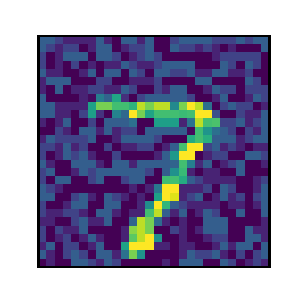
\includegraphics[width=.225\textwidth]{Fig1.eps}
    \caption{A `7' perturbed with adversarial noise such that the model perceives it to be a `2.'}
    \label{fig:attack}
    } % end centering
\end{figure}
% % Noisy Number

\paragraph{Attack Distance}
\begin{figure*}[!ht]
    {\centering
    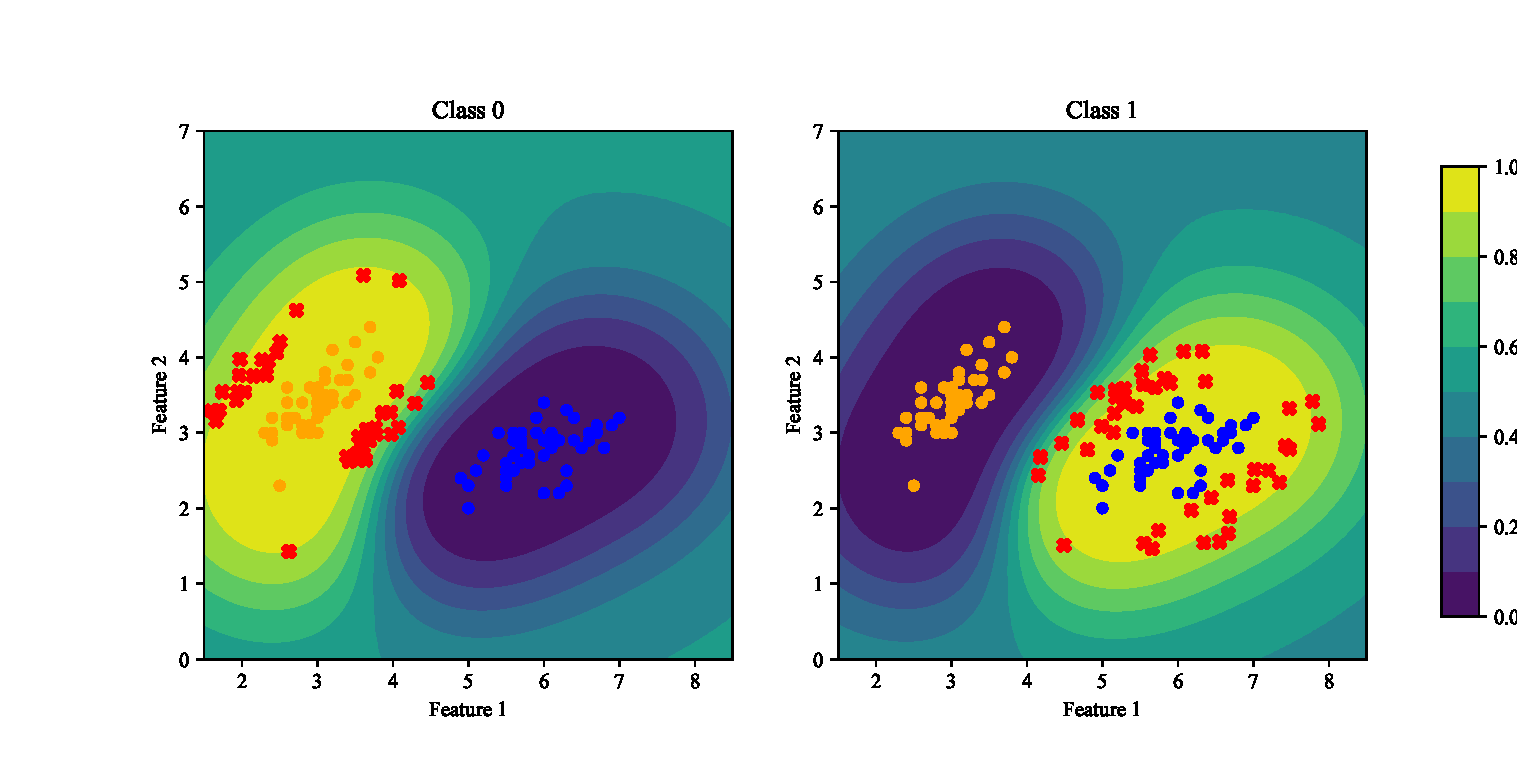
\includegraphics[,clip,width=0.9\textwidth]{Fig2.eps}
    \caption{Orange (class 0) points, blue (class 1) points, and red (adversarial) points in a contour map for a radial basis function support vector classifier. The contours reflect the confidence levels for a given sample and class. The bright yellow regions indicate areas of strong positive confidence and the purple areas indicate strong negative classification, and grey represents an uncertain classification. As we can see, it is rather trivial to shift the classification of a given sample \cm{towards} the ambiguous regions (teal colored).}
    \label{fig:shift}
    } % end centering
\end{figure*}

Figure~\ref{fig:shift} depicts a radial basis function support vector machine, classifying the points into orange (class 0) or blue (class 1). However, the red points indicate successfully generated adversarial examples. Figure~\ref{fig:attack} shows an example of a `7' that has added adversarial noise such that the classifier sees it to be a `9'. 
In related surveys~\cite{dohmatob_generalized_2019, biggio_evasion_2013-1, bect_bayesian_2017, chakraborty_adversarial_2018, carlini_towards_2017, croce_reliable_2020}, a model's adversarial robustness is defined as its performance accuracy against a given adversary. A thorough examination of such attacks are explored in Section~\ref{attacks} below, but, in general, an attacker perturbs an image such that the perturbation distance, $d$, is less than or equal to a threshold value, $\epsilon$, specified by the experimenter, under some conception of distance. The evaluations in this study examine both the $\ell_{\infty}$ and $\ell_2$ norms for the gradient-based attacks and $\ell_1$ in other contexts, which consider perturbations no larger than $\epsilon$, where $\ell_{\infty}$ and $\ell_2$ allow for perturbations across the entire feature space, and $\ell_0$ restricts the number of perturbed features. In our study, we restrict this perturbation distance to be 1 byte, as is typical in the literature \cite{madry2017towards, miller_adversarial_2020, biggio_evasion_2013, biggio_multiple_2009}. 

\paragraph{Attack Strength}
 Since adversarial perturbations, by definition, are the perturbations that maximizes the model loss through various methods, each approximates a different worst-case scenario. The `strength' of an attack is generally related to the magnitude of these perturbations~\cite{carlini_towards_2017}, and is measured by retrospective evaluations of model accuracy in which a `strong' attack induces more loss. It is necessary to evaluate against the strongest possible attack for a given model and data set, but the strength of an attack is always contextual, since the magnitude of a perturbation must be measured with respect to some normed vector space, is specified in advance, and subject to real-world constraints. Additionally, we know that models optimized to prevent one attack do not necessarily generalize to other attacks~\cite{carlini_towards_2017}, especially across distance metrics. 


\subsection{Defenses}
% Note to editors: This was just moved from a lower section to compensate for a shuffling of chapters. The text remains substantially the same.
The attacks outlined above are capable of breaking state of the art image recognition models.  However a variety of defenses have been proposed that act on the dataset or the model output. Those broadly fall into categories that seek to identify an attacker and isolate them from the model API, ones that seek to isolate tainted examples from the database, or ones that attempt to mitigate all potential attacks during run-time. Below, we outline a wide variety of defenses proposed over the last several years and measure their effect on the failure rate of various models. We have excluded model transformation defenses and secondary detection models since those sidestep the problem of making a given model more robust and do nothing for the IEC requirement that each electro-mechanical component meets the regulatory standard in isolation from each other component (see Section~\ref{safety-critical}).


% \paragraph{Critical Attack Distance}

% \cm{
% In general, as proven by Dohmatob~\cite{dohmatob_generalized_2019}, for all classifiers that map $p$ features to $k$ classes ($\mathbb{R}^p \mapsto \mathbb{R}^k $), there is a critical distance ($\ell_{\infty}$ norm) for which all classifiers can be fooled with high probability defined by:
% \begin{equation}
% \epsilon_{\infty} := \sigma_k \sqrt{\frac{2 \log (\frac{1}{\eta })}{p}},
% \label{dohmatob}
% \end{equation}
% where $\eta$ is the probability of finding a misclassified example and $\sigma_k$ is the covariance matrix of input $x \in \mathbb{R}^P\mapsto \mathbb{R}^k$. Its clear that the predominant component of this critical distance is the signal noise $\sigma_k$, followed by the number of features $p$, which correspond to the signal noise ($\sigma_k$) and the number of features ($p$) for a given model's input, but could just as easily apply to the signal and feature space of a single layer.
% }

% See Figure~\ref{fig:dohmatob} to see the sensitivity analysis of these variables. 
% Marginal gains in accuracy ($1 - \eta$) are offset by small changes in the resolution ($p$) or random noise ($\sigma_k$).
% % TODO: Figure
% \begin{figure}
%     \centering
%     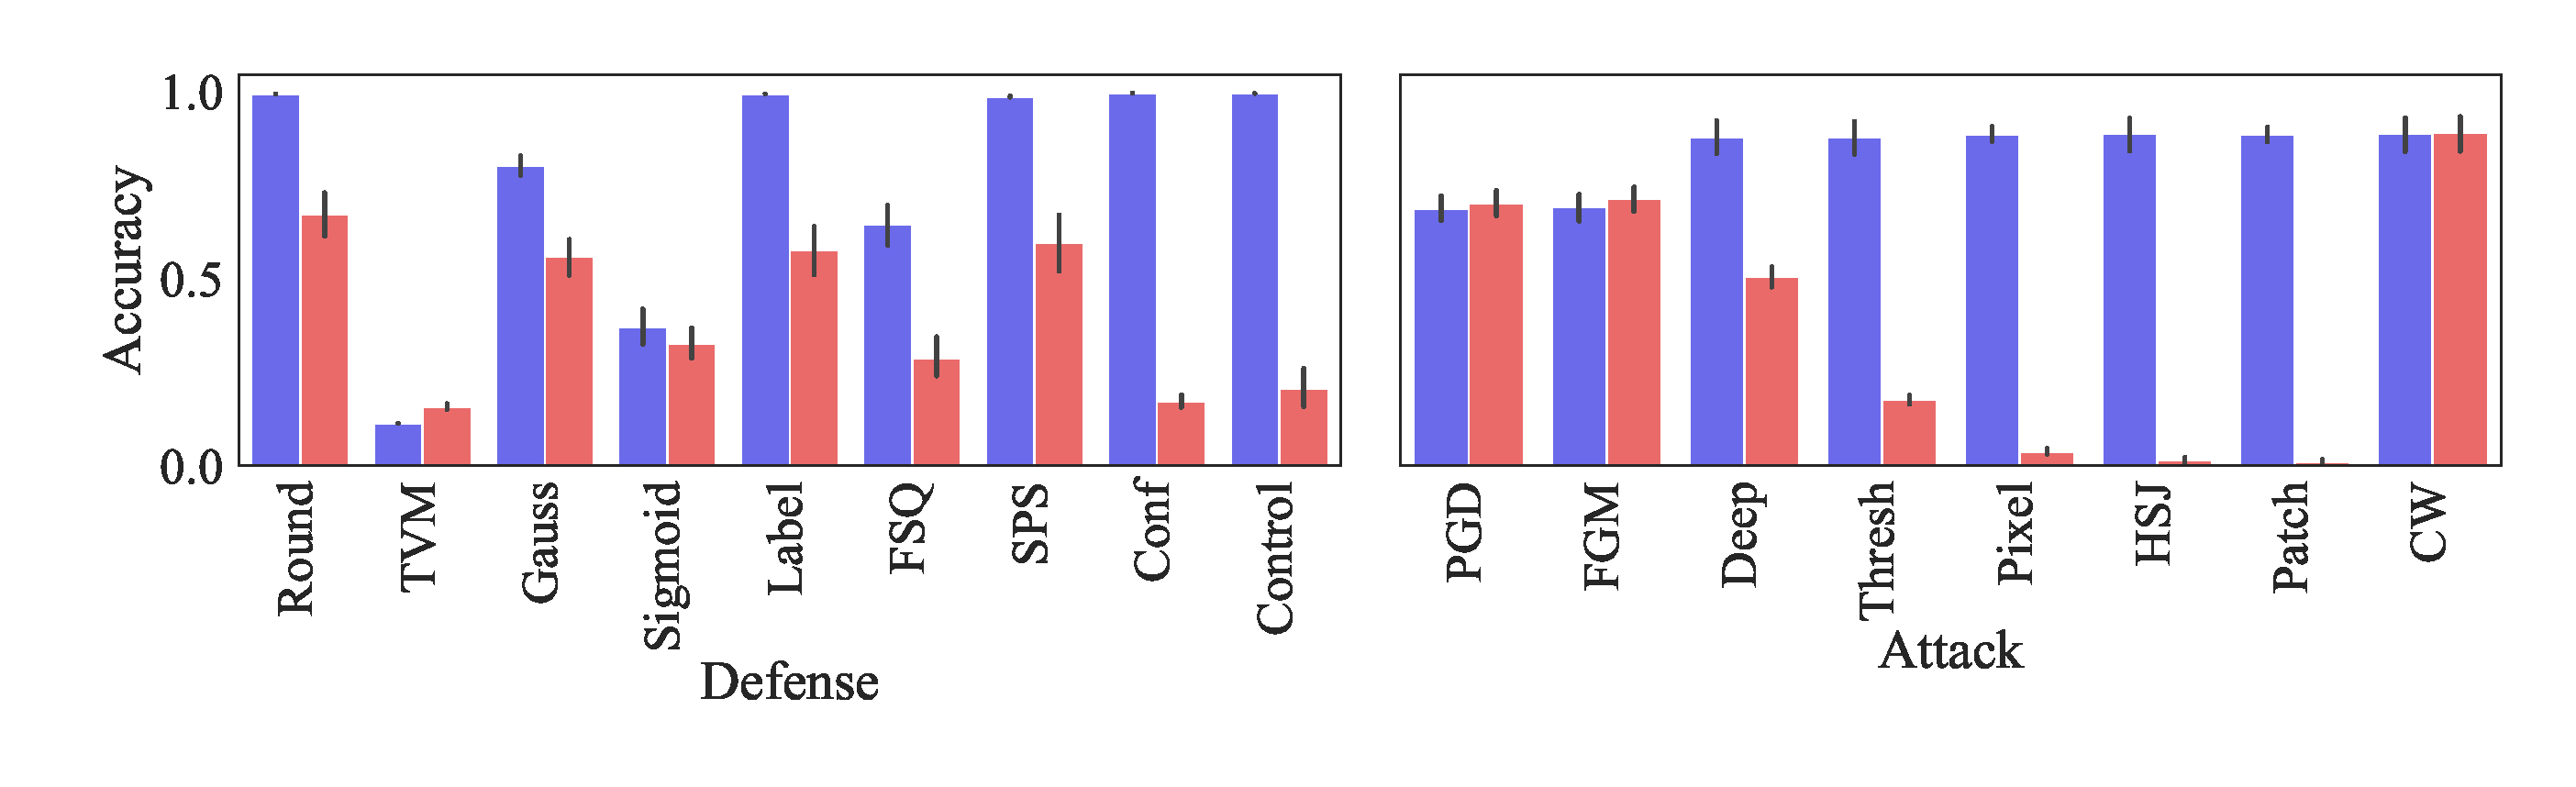
\includegraphics[width=.4\textwidth]{accuracy_plot.eps}
%     \caption{This figure shows how the critical adversarial distance (y-axis) varies with respect to the accuracy for MNIST (solid) and CIFAR-10 (dotted). TODO}
%     \label{fig:dohmatob}
% \end{figure}


\subsection{Attacker's Knowledge}
 While the general assumption is that an attacker has whitebox access to an entire pipeline (including data, model weights, and output), that does not necessarily need to be the case~\cite{hopskipjump, chakraborty_adversarial_2018}. While some attacks do need whitebox access, prior research~\cite{hopskipjump, nelson2010behavior} has shown that a surrogate model and data-set can be used to approximate $K$ using a proxy model $\widehat{K}$, built using the class labels provided by the model at test-time, that is sufficient for creating strong adversarial examples. Tram\`er \textit{et al.}~\cite{tramer2016stealing} examined popular machine learning as a service platforms that return confidence values as well as class labels, showing that an attacker can build a proxy model by querying $ p + 1$ random $p-$dimensional inputs for unknown $p+1$ parameters. Further research~\cite{fredrikson_model_2015} was able to reverse engineer the training data-set through black-box attacks against a model that returns confidence levels, with the caveat that the inferred data might be a meta-prototypical example that does not appear in the original dataset. 

Fortunately for our attacker, such examples are still useful for determining the underlying data distribution, even if they manage to preserve some of the privacy of the original dataset. Shokri \textit{et al.}~\cite{shokri2017membership} presented a membership inference attack that determines whether a given data point belongs to the same distribution as the original training data using a set of proxy models.  Below, we examine the efficacy of several attacks from the perspective of loss as well as the functional query bandwidth.



\subsection{Metrics}

\cm{[Note: This subsection has been moved. It was previously before the adversary and defence sections.]}

\label{metrics}
The ISO standards \cite{iso26262} define the \cm{Safety Inegrity Level (SIL)} in failures/per hour, which we have converted to failures per second in Table~\ref{tab:rate}. If assume that \textit{accidental} adversarial errors are possible in real-world systems due to things like dust, lens flare, component failure, packet loss, \textit{etc.}, it naturally follows that the adversarial failure rate is an estimate of the models behavior at the edge or in the `worst-case scenario'. That is, the \textit{adversarial failure rate} is an estimate of the upper bound of the real-world failure rate in adverse but otherwise mundane circumstances. 




\paragraph{Accuracy}

The accuracy is defined as
\begin{equation}\label{eq:accuracy} 
    % \mathrm{Failure~rate}
    \mathrm{Accuracy}
    = 1 - \frac{\mathrm{False~Classifications}}{\mathrm{Total}}
    = 1 - \eta,
\end{equation}
where \textit{Total} is the number of tested samples, \textit{False Classifications} refers to the number of objects that were incorrectly categorized by a given model[, and $\eta$ is the generalized error rate. In practice, $\eta$ is generally assumed to be the accuracy on a `test set', with samples from a distribution assumed to be identical to the training set. Elsewhere, we refer to this `test set' accuracy as the 'benign' accuracy or with the subscript `ben.' such that the test accuracy is $\eta_{ben.}$. In addition to this metric, we include metrics for a variety of signal processing techniques (see: Section~\ref{defenses}) where the unaltered signal is designated as `control'. Finally, we include many sets of test sets specifically crafted to be `adversarial' (see: Section~\ref{attacks}), which are denoted with the subscript `adv.'.

However, due to the large number of samples required by regulatory standards  and the strenuous testing requirements of safety-critical software (see Section~\ref{safety-critical}), these evaluations become an infeasible way to verify that a model only fails once across the required number of samples (see Table~\ref{tab:rate}), especially if we would like to be highly confident of that estimation.

\begin{table}[!ht]
    \begin{center}
        \caption{Acceptable Failure Rates for different SIL levels in which a single death is possible, measured in failures per second.}
        \begin{tabular}{l c cc}
            \toprule
            SIL  && On-demand Operation   & Continuous Operation \\
            \cmidrule{1-1} \cmidrule{3-4}
            I     && $[10^{-6}, 10^{-5})$  & $[10^{-10}, 10^{-9})$ \\
            II    && $[10^{-7}, 10^{-6})$  & $[10^{-11}, 10^{-10})$ \\
            III   && $[10^{-8}, 10^{-7})$  & $[10^{-12}, 10^{-11})$ \\
            IV    && $[10^{-9}, 10^{-8})$  & $[10^{-13}, 10^{-12})$ \\
            \bottomrule
        \end{tabular}
        \label{tab:rate}
    \end{center}
\end{table} 


\paragraph{Failure Rate}

Instead of evaluating every software change in our pipeline against the legally required $[10^7,10^{12})$ number of samples, we can measure the precise failure rate (elsewhere $\lambda$) with a much smaller number of samples if we measure it with



\begin{equation}\label{eq:failure_rate}
    \mathrm{Failure~Rate} = \frac{\mathrm{False~Classifications}}{\mathrm{Total ~Time~(s)}}
                          = \lambda,
\end{equation}
where \textit{False~Classifications} is the number of misclassified samples, and \textit{Total time} refers to the total time it takes to classify all the samples. 


\subsection{Robustness}
\textit{Robustness}, then, is a measure of how well a model resists these \textit{induced} failures. In this survey, we examine how several different model and data transformations (see Section~\ref{defenses}) influence this property for a given model architecture and dataset. We measure the efficacy of a given model change, using the \textit{Percent Change in Accuracy} ($\%\Delta ACC$):

\begin{equation}
    \label{eq:percent_change_acc}
    \mathrm{\%\Delta ACC = 
        \frac{Acc.-Control~Acc}{Control~Acc}} \cdot 100
\end{equation}

where $Acc$ refers to the \textit{accuracy} as defined in Eq.~\ref{eq:accuracy} and $Control$ refers to the performance of the unchanged model on the benign ($Ben.$) dataset. This measures the marginal risk of failure for a particular model change (defense) in the adversarial case when compared to the benign case. We also defined the the metric \textit{Relative Change in Failure Rate ($ \Delta \lambda$):}

\begin{equation}
\label{eq:relative_change_failure_rate}
\mathrm{\Delta \lambda} = 
    \frac{\mathrm{\lambda_{control}-~\lambda}}{\mathrm{\lambda}}
\end{equation}
where $\lambda$ refers to the failure rate, $Control$ refers to the unchanged model. Taken together, these two metrics allow us to measure the marginal risk of a given defense in both the benign and adversarial circumstances. In both cases, a positive number indicates an improvement in relative risk and a negative number indicates a worsening of relative risk, Eq.~\ref{eq:percent_change_acc} in the context of accuracy and Eq.~\ref{eq:relative_change_failure_rate} in the context of failure rate.




% \footnote{By estimating this probability (or a vector of them), we can model this failure rate as a function of time. This kind of analysis is quite common in the medical and manufacturing sectors, called `accelerated failure time' models~\cite{aft_models}. By modelling this failure rate using an exponential distribution, where time, $t$, is measured in seconds, we get
% $S(t) = \theta \lambda e^{ -\theta \lambda t}$
% with an \textit{expected} \textbf{survival time} ($S(t)$) of
% $$
%     S(t)= \frac{1}{\theta \lambda} \mathrm{~seconds}
% $$
% an \textit{expected} \textbf{failure rate} of 
% $\eta \approx \theta \lambda  \mathrm{~failures~per~second}$
% in the simplest case.  The convenience of this methodology is that it allows us to model generalized error according to well-known probability distributions. With the inclusion of other measured or estimated parameters, we could also be model this as log-normal, Weibull, or generalized-$\gamma$ distributions~\cite{aft_models}. However, in our results, we show that the failure rate is so large that the choice of model here scarcely matters.} 





% The Ornstein isomorphism theorem says that any two such schemes are isomorphic (\ie, have the same decision boundaries) if an only if they have have the same entropy. That is to say, $H(\probP_1) = H(\probP_2) \iff p_1 \mapsto p_2 \forall p_1, p_2 \in P_1, P_2$. In other terms, being able to successfully describe everything that is not a cyclist is bijectively equivalent (e.g \textit{isomorphic}) to being able to precisely and accurately describe a cyclist. Therefore, in order to minimize the uncertainty in the general case, we must at least minimize it in the adversarial case.

% \cm{A corollary to the above theorem is that there is a unique flow with infinite entropy, but I can't conceptualize what a `flow' is outside of thermodynamics. This seems like an important realization when paired with the `maximum entropy principal' (MEP)}

%\cm{By definition, an attack attempts to maximize the cross-entropy loss, which is the opposite goal of the model. Here the MEP seems like an important realization as well.}






\subsection{Hyperparameter selection}

For many attacks, hyper-parameters such as the targeted false confidence threshold, step size, batch size, number of iterations, and distortion norm must be specified in advance by the attacker~\cite{carlini_towards_2017}. Furthermore, because many of these are drawn from a continuous (and therefore infinite) space, finding a strong attack is computationally expensive and finding the strongest possible attack is at least NP-Hard~\cite{carlini_towards_2017}, with the problem exacerbated by the extreme non-linearity of CNNs. Even more concerning, there is not yet a mathematical foundation for what constitutes a `good' attack, relying only on after-the-fact evaluations of model accuracy. By examining a large hyper-parameter space, we demonstrate how each defense generalizes across the feasible attack spectrum rather than relying on a single canonical evaluation metric.

\subsection{Attack and Defense Cost Analysis}

Like in cryptography, the fundamental limit for an adversary has to do with computational cost~\cite{hoffstein_pipher_silverman_2010}. For example, model inversion attacks become pointless if it is computationally more expensive to steal a model than it is to train one. Likewise, model defenses are only as useful insofar as they have the ability to be deployed in existing real-time systems. As such, we examine the cost of various defenses as well as the number of queries and query rate of various attacks. The best modern methods are limited to computationally expensive techniques like reject on negative impact~\cite{nelson2010behavior}, Bayesian subset analysis~\cite{bect_bayesian_2017}, and model post-processing techniques that degrade accuracy with added computational cost~\cite{athalye_obfuscated_2018, papernot, li_general_2016}, making them unsuited for the task of improving our ability to reliably generalize. For most attacks, we tested the perfect knowledge scenario, but we have also included the `HopSkipJump' attack~\cite{hopskipjump} to model the worst case for an attacker that only has access to a standard machine learning application programming interfaces (APIs) which only exposes hard class labels.


\section{Attacks}
\label{attacks}

\cm{The following section outlines a variety of attacks, broken into three categories: gradient-based attacks, gradient approximating attacks, and universal attacks. For the sake of the reader, a collection of generated adversarial samples follows the mathematical descriptions in the subsection following the aforementioned trio (see:~Sec.~\ref{samples}).}

\subsection{\cm{Gradient-Based Attacks}}

\cm{
The seminal work on adversarial attacks in the context of modern neural networks was written by Madry~et~al.~\cite{madry2017towards} and an important follow up work was written by Carlini~and~Wagner~\cite{carlini_towards_2017}. Both operate under the condition that the attacked model has a gradient that is known to the attacker. Each of these can be considered \textit{white-box} attacks because they are given access to the model output and the model gradient. 
}


\subsubsection{FGM}

The fast gradient sign method (FGM)~\cite{fgm} is the most basic and fastest such attack. It is defined by the step,
$$
   \widetilde{x} = x + \epsilon \cdot \textrm{sgn}\Big(\nabla_{x} L\big(y, K(x)\big)\Big),
$$
where $L$ is the loss function, as described above, $\nabla_{x} L$ is the gradient of $L$ with respect to the input $x$, the $\epsilon$ is the maximum perturbation distance, $\textrm{sgn}$ is the element-wise signum function, and $\widetilde{x}$ denotes a generated adversarial sample. It is called `fast' because it does not check the feasibility of the perturbation (if it is within a maximum distance, $\epsilon$, as is done in other methods, see \eg~PGD below).

As such, it may not be as successful as other methods, but operates very quickly. We tested several different step sizes and norms for this method, enumerated in Figures~\ref{fig:adv_acc_grid}~and~\ref{fig:mnist_adv_acc_grid}. 

\subsubsection{PGD}

Projected gradient descent (PGD)~\cite{carlini_towards_2017} takes a gradient step to increase the loss, but also includes a projection step, $\mathrm{Proj}_\epsilon$, that enforces the constraint of a perturbation distance q of at most $\epsilon$ with respect to some norm by projecting onto the feasible set (defined by the perturbation distance, $\epsilon$). The iteration scheme of PGD is
$$
    x^{(s+1)} = \mathrm{Proj}_\epsilon \Big( x^{(s)} + r \cdot \nabla_{x^{(s)}} L\big(y, K(x^{(s)})\big) \Big),
$$
where $r$ is a step size, $s$ is a sequence index, and $x^{(S)}$ denotes a generated adversarial sample after $S$ steps. This iteration is repeated until a specified number of iterations, $S$, have been reached. The number of iterations is specified by the attacker, which ultimately determines the processing-time against a given model, scaling linearly with the number of iterations. We tested several different step sizes and norms for this method, enumerated in Figures~\ref{fig:adv_acc_grid}~\&~\ref{fig:mnist_adv_acc_grid}. 

\subsubsection{Carlini--Wagner}

Carlini and Wagner (CW)~\cite{carlini_towards_2017} devised an attack that minimizes the perturbation distance subject to a distance constraint while maximizing the false confidence.
The iteration scheme is for some constant, $C$,
$$
    x^{(s+1\hspace{-0.025em})}\hspace{-0.2em}=\hspace{-0.15em}\argmin_x \hspace{-0.1em} \|x^{(s)} - x\|_2^2 + C \hspace{-0.05em} \max\hspace{-0.15em}\big(\hspace{-0.15em}\max_{j\neq t} g_j(x) - g_t(x) + C, 0\big)
$$
where the $g_j, g_t$ are discriminant functions and the goal is to minimize the perturbance with a penalty for not changing it to the target class. It also generalizes beyond the squared $\ell_2$ norm. This method attempts to enforce attack quality by penalizing examples with low confidence and continuing to iterate on them until either a maximum number of iterations or the specified false confidence is reached. For our tests, we used the $\ell_{\infty}$ norm and a confidence threshold of 99\%. 

\subsection{\cm{Gradient-Approximating Attacks}}

\cm{
Further work sought to find attacks that did not rely on explicit gradient information. The \textit{Deepfool} attack~\cite{deepfool} uses a quadratic approximation of the boundary condition to generate a separating hyperplane, while \textit{Few-Pixel} and \textit{Threshold}~\cite{pixelattack} use a search algorithm known as differential evolution rather than relying on explicit gradient information. Each of these attacks can be considered \textit{grey-box} attacks because they rely on un-categorized model output but use that output to approximate the gradient, rather than rely on explicit access to the model weights.
}



\subsubsection{DeepFool}

The DeepFool attack~\cite{deepfool} seeks to find the smallest perturbation that causes a misclassification using a first-order Taylor approximation of the classifier. In essence, it seeks to find the minimal separating hyperplane between the target sample's true class and another. It assumes that it has access to the entirety of the model, including the confidence level (expressed as a logit) of all labels, the true label of a sample ($x$) and the model gradient. The iteration scheme is
$$
    x^{(s+1)} = \argmin_x \|x^{(s)} - x\|_2 
$$
subject to 

$$
f(x^{(s)}) + \nabla_{x^{(s)}} f(x^{(s)})^T(x^{(s)} - x) = 0,
$$
with $\|\cdot\|_2$ is the $\ell_2$ norm, and where $f$ outputs the logits of $K$, such that $K(x) = \phi(f(x))$, with output activation, $\phi$. Run-time is determined largely by the number of iterations, $S$, and the number of gradients $w.r.t.~L(x)$ used to estimate $f(x)$, which we set to 10 such that the gradient was calculated for each class. The existence of any such attacks with a distance than or equal to some some specified robustness threshold ($\epsilon \leq \epsilon_{critical}$) should immediately cause concern.

\subsubsection{Few-Pixel}

The few-pixel attack~\cite{pixelattack} (Pixel) attempts to maximize the loss by iteratively finding the least robust pixel set and perturbing it by less than some specified threshold, $\epsilon$. 
That is, this attack seeks to maximize false confidence while minimizing the number of perturbed pixels.
The iteration scheme is
$$
    x^{(s+1)} = \argmax_r \, L\big(y, K(x^{(s)} + r)\big) \text{~~subject~to~~}  \|r\|_0 \leq \epsilon,
$$
where $r$ is the perturbation and $\epsilon$ is the perturbation distance in pixels, typically of just one pixel. This attack uses differential evolution to simultaneously optimize for both loss and the number of perturbations. In our case, we limited this to a single perturbation, but did not restrict epsilon beyond the normal $[0, 255]$ range. Since perturbation distance for a single pixel is not restricted, we restricted the number of distorted pixels to one of these: $[1,2,4,8, 16]$. \cm{Unlike the aforementioned gradient-based attacks, this method generalizes to classification systems that lack gradients (\textit{e.g.}, decision trees). This differs from the the \textit{Threshold} and \textit{Adversarial Patch} attack below by optimizing for the fewest number of changed pixels ($\ell_0$ norm) rather than the perturbation distance ($\ell_2$ or $\ell_{\infty}$).}

\subsubsection{Threshold}
The threshold attack~\cite{pixelattack} is similar to the few-pixel attack (in that it uses differential evolution as the optimization algorithm), but uses the $\ell_{\infty}$ norm rather than the $\ell_0$ distance. This method, like the Carlini Wagner (CW) method, attempts to generate examples that are both false and highly confident. However, it uses a complicated algorithm (differential evolution) rather than simple, linearized methods (as in CW). The iteration scheme is
$$
    x^{(s+1)} = \argmax_r \, L\big(y, K(x^{(s)} + r)\big) \text{~~subject~to~~}  \|r\|_{\infty} \leq \epsilon
$$
where $\epsilon$ is the targeted perturbation threshold of .03. \cm{Unlike the aforementioned gradient-based attacks, this method generalizes to classification systems that lack gradients (\textit{e.g.}, decision trees). This differs from the the \textit{Few-Pixel} and \textit{Adversarial Patch} attack below by optimizing for largest change in loss ($\ell_{1}$ norm) rather than fewest number of pixels ($\ell_{0}$ norm) or the perturbation distance ($\ell_2$ or $\ell_{\infty}$). }

\subsection{\cm{Universal Attacks}}
\label{universal}
\cm{
Even further work has sought to go beyond computationally-intensive approximations for each attacked sample or model query. The \textit{Adversarial Patch technique}~\cite{adversarialpatch} uses the aforementioned differential evolution algorithm to generate an additive noise sample that maximizes the loss \textbf{for all samples} and is considered a \textit{grey-box} attack because it relies on un-categorized model outputs but not explicit access to the model weights. However, we include it here because the nominal image patches generated by this technique are meant to generalize to unseen data as the number of API queries increases, meaning that this can be trained using data wholly disconnected from the model-builder's dataset. The \textit{HopSkipJump} attack~\cite{hopskipjump} has been shown to minimize the number of API queries required to break \textbf{any model}. As such, it is considered a \textit{black-box} attack. 
}


\subsubsection{Adversarial Patch}

The Adversarial Patch attack~\cite{adversarialpatch} (Patch) uses the same differential evolution algorithm as the Threshold Attack. However, instead of optimizing for a threshold or confidence level, it seeks to change each class into any other by applying an image patch that is not unique to a given image, but is universal for a  given dataset. This single generated image patch is added to each image and is intended to cause a generic misclassification, regardless of the original class.  We know that these attacks are quite general for a given dataset and not specific to a given model \cite{adversarialpatch, xiao2021improving}, raising serious concerns about an attacker's ability to generate universal and offline attacks for a given set of data. Like with the Pixel attack, the per-pixel distortion is not restricted, so we restricted perturbation to a percentage of the benign image, using the hyper-parameters [.03, .1, .25, .5, 1.0].  \cm{Unlike the aforementioned gradient-based attacks, this method generalizes to classification systems that lack gradients (\textit{e.g.}, decision trees). This differs from the the \textit{Threshold} and \textit{Adversarial Patch} attack below by optimizing a single perturbation that works for every image rather than minimizing the geometric perturbation distance ($\ell_2$ or $\ell_{\infty}$ norm) while minimizing the number of pixels required for said universal patch ($\ell_0$).}

\subsubsection{HopSkipJump}

The HopSkipJump attack~\cite{hopskipjump} (HSJ) is a query-cost-aware model that acts on hard class labels rather than confidence levels (\ie, a blackbox attack). It finds a point on the boundary (using binary search between the initial attacked point and a point on the other side of the decision boundary), and approximates the gradient at the boundary using Monte Carlo sampling in an offline manner. Then, a step is taken in the approximated gradient direction, the model is queried again with the new points, and the process is repeated. The procedure iterates the step,
$$
   x^{(s+1)} = \mathrm{Proj}_{\epsilon,x^{(0)}}\Bigg( x^{(s)} + r^{(s)} \frac{\widetilde{\nabla}_{x^{(s)}}  Q(x^{(s)}) }{\big\|\widetilde{\nabla}_{x^{(s)}} Q(x^{(s)}) \big\|_2}\Bigg),
$$
where $x^{(s)}$ is an adversarial sample, $s$ a sequence index, $\mathrm{Proj}_{\epsilon,x^{(0)}}$ is an $\ell_2$ projection of a point onto a sphere of radius $\epsilon$, centered at the initial point $x^{(0)}$, and $\widetilde{\nabla}_xQ(x)$ is the Monte Carlo estimate of the gradient of $Q$ at $x$, and
$$
    Q(x) = \max_{c\neq c^*} K_c(x) - K_{c^*}(x),
$$
where $K_{c}$ is the model output for class $c$, and $c^*$ is the class of the initial point, $x^{(0)}$. This attack's run-time is controlled by the number of (offline) gradient estimations, the number of random samples per (online) query, and the number of iterations of both parts of the algorithm. This attack finds an adversarial example that is close ($\epsilon \leq \epsilon_{critical}$) to the original sample, but still causes a misclassification.  This model is query efficient as it uses a small number of API queries to approximate the gradient and then uses this information to approximate the gradient near the class boundary and optimize the perturbation distance of the attacked sample. Also, because this attack approximates the gradient rather than relying on explicit whitebox access to it, it can be used to attack non-differentiable models (\eg random forests). That is, this is one of the most universal black box attacks.

\subsection{Attack Samples}
\cm{
To aid the reader, we have visualized a single attack sample for each attack on the undefended (control) model, depicted in Figures~\ref{fig:FGM}-~\ref{fig:HSJ}. Additionally, we have provided the failure rate, $\eta$, defined in Eq.~\ref{eq:failure_rate}, and tested on 100 samples from the MNIST dataset. For each attack, we also vary a distance parameter, determined by the optimization criteria for each attack outlined above. For the sake of clarity different distance metrics are denoted with a distance of $epsilon$ subject to some norm, $| \cdot |_n$ such that $\ell_2$ norm of ${\epsilon}$ is $ | \epsilon |_2$
}

\label{samples}
\begin{figure*}[]
    %\begin{subfigure}
          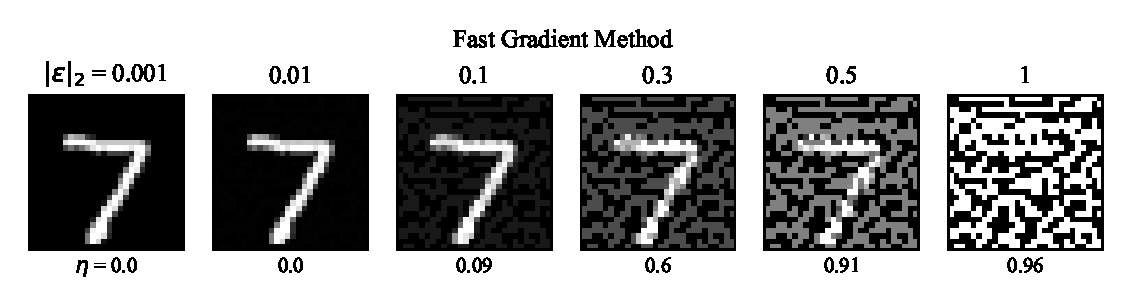
\includegraphics[,clip,width=0.9\textwidth]{Fig3.eps}
        \caption{ \cm{ The Fast Gradient Method (FGM) doesn't enforce any kind of feasibility criteria, resulting in salt-and-pepper noise as the $\ell_2$ approaches the standard deviation of the normally distributed dataset.}}
        \label{fig:FGM}
     %\end{subfigure}
     %\begin{subfigure}
          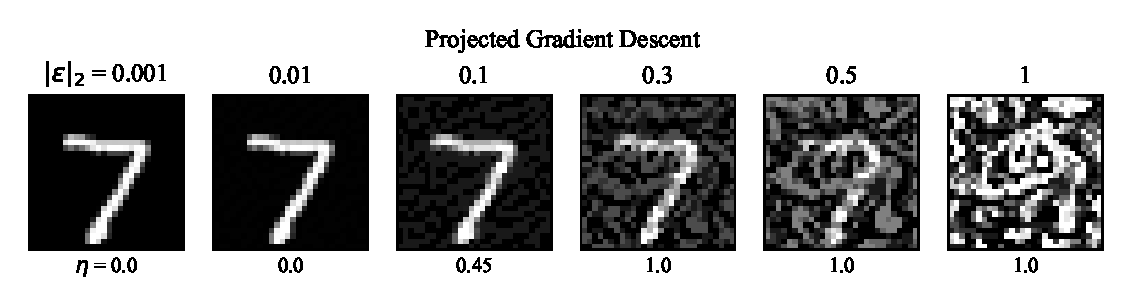
\includegraphics[,clip,width=0.9\textwidth]{Fig4.eps}
        \caption{ \cm{The Projected Gradient Descent Attack (PGD) projects the adversarial example back onto a sphere of a fixed radius, yielding noise that more closely approximates handwritten digits.}}
        \label{fig:PGD}
     %\end{subfigure}
     %\begin{subfigure}
          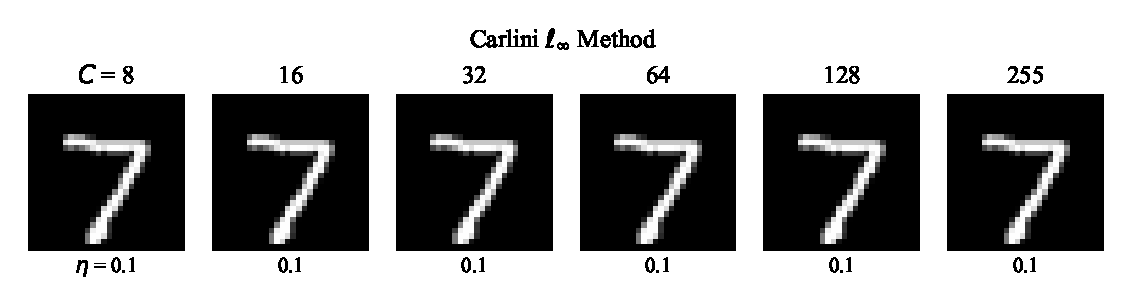
\includegraphics[,clip,width=0.9\textwidth]{Fig5.eps}
        \caption{ \cm{The Carlini-Wagner $\ell_{\infty}$ method includes an added confidence constraint that only returns an adversarial example $\iff L(x^{s+1}) - L(x) \geq C$. Depicted here is the unperturbed 7 because this method was unable to find an adversarial example for these constraints. Despite this, we can see that for 10\% of the samples are consistently misclassified with a high degree of false confidence. 
        }
        }
        \label{fig:CW}
     %\end{subfigure}
     %\begin{subfigure}
          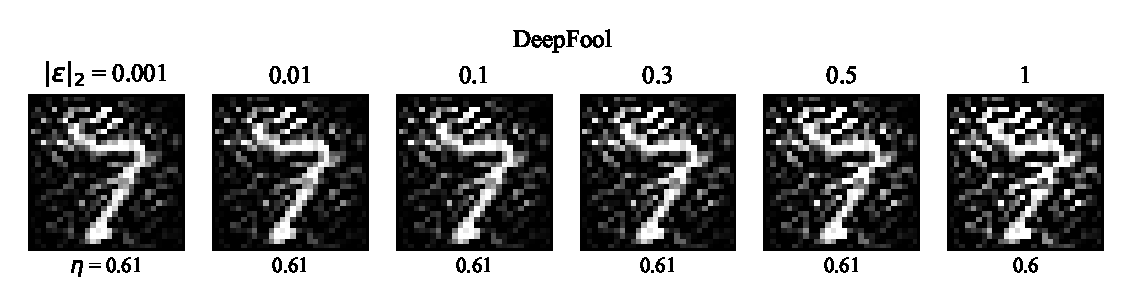
\includegraphics[,clip,width=0.9\textwidth]{Fig6.eps}
        \caption{\cm{The DeepFool Method, rather than constraining perturbations to an $\epsilon$-sphere around the sample, finds perturbations that extend beyond the approximated boundary by a distance of at least $\epsilon$. Regardless of the distance constraint, DeepFool is very effective.}}
        \label{fig:Deep}
     %\end{subfigure}
 \end{figure*}


\begin{figure*}[] 
    %\begin{subfigure}
          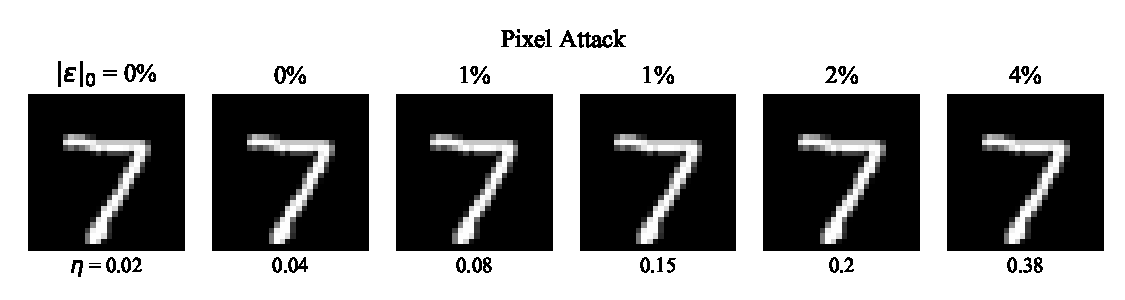
\includegraphics[,clip,width=0.9\textwidth]{Fig7.eps}
        \caption{ \cm{The Pixel Attack (Pixel) seeks to maximize the loss while minimizing the number of perturbed pixels. Here we see that even a small  perturbation in original image can lead nevertheless consistently induce failures.  Here, $\epsilon_0$ denotes the ratio of perturbed pixels to the total.}}
        \label{fig:Pixel}
     %\end{subfigure}
     %\begin{subfigure}
          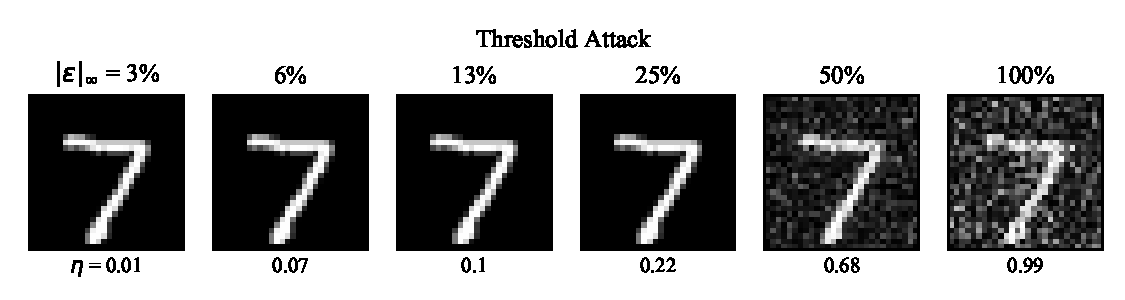
\includegraphics[,clip,width=0.9\textwidth]{Fig8.eps}
        \caption{ \cm{Rather than minimizing the number of pixels, the Threshold Attack (Thresh) optimizes for the smallest perturbation possible. Here, $\epsilon_{\infty}$ denotes the ratio of the applied to noise to the maximum possible value (255).}}
        \label{fig:Thresh}
     %\end{subfigure}
     %\begin{subfigure}
          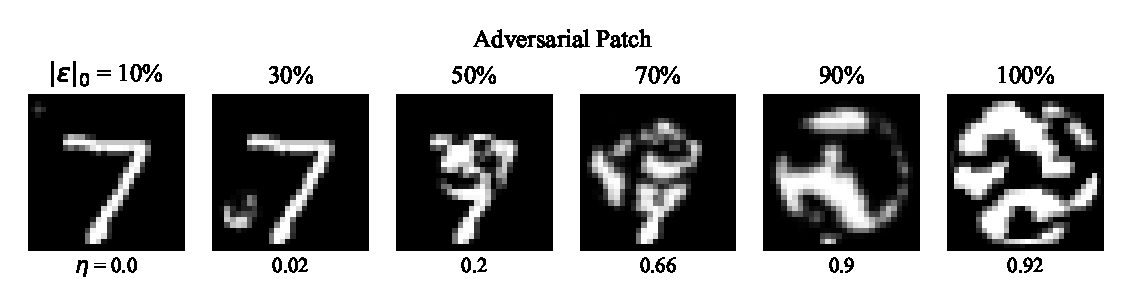
\includegraphics[,clip,width=0.9\textwidth]{Fig9.eps}
        \caption{ \cm{ This is one of the two most dangerous attacks as it can consistently find image patches (the noisy circle depicted above) from only a small number of samples ($n=100$) that can often fool the classifier, regardless of original image or class. Obviously, as we replace all of the pixels with adversarial noise, the classifier becomes mostly useless, but this attack is still concerningly effective when only a fraction of the image has the adversarial noise. Here, $\epsilon_0$ denotes the ratio of perturbed pixels to the total.}}
        \label{fig:Patch}
     %\end{subfigure}
     %\begin{subfigure}
          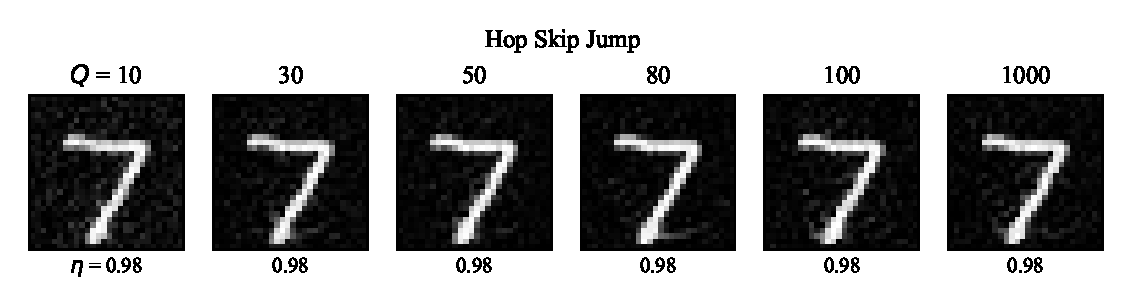
\includegraphics[,clip,width=0.9\textwidth]{Fig10.eps}
        \caption{ \cm{The Hop Skip Jump Attack (HSJ) uses a second-order approximation of the classification boundary in an offline manner to find adversarial examples that first maximize loss then minimize for perturbation distance. This attack is uniquely concerning because it 1) works on any model and 2) is surprisingly effective even when our attacker is restricted to a small number of queries per batch (here, denoted as $Q$).}}
        \label{fig:HSJ}
     %\end{subfigure}
\end{figure*}



\section{Defenses}
\label{defenses}




\subsection{Attacker Identification}

We must assume that at least some of the user inputs will `adversarial', even if that adversary is sensor failure and not an intentional attack. Identifying and isolating this adverse input may not require a perfect anomaly detection system, but could draw from graph theoretical representations to identify and isolate networks of distributed attackers, allowing the model API provider to revoke access or otherwise isolate the attack effects from the models. While this has been done in the context of social networks~\cite{daya_graph-based_2019}, these techniques can easily be fooled with intermittent attacks~\cite{intermittent}, distributed attacks~\cite{distributed_attacks}, or something as simple as a quadratic approximation of the model~\cite{hopskipjump}. For web services more generally, legitimate users are often identified by using CAPTCHA~\cite{ahn2003captcha}, but that it not a solution for an API meant to be accessed by software. Furthermore, outsourcing this to a secondary component would run afoul of the IEC requirement that each component meet regulatory standards in isolation from all other components (see Section~\ref{safety-critical}). However, even if we assume all samples are generated by legitimate users with guaranteed data integrity, we still cannot be confident that `adversarial' noise will not be generated inadvertently by routine phenomena like sensor failure, dust, low-light conditions, lens aberration, precipitation, or another mundane cause. One possible approach is to eliminate `bad' samples at run-time.

\subsection{Subset Analysis}

Subset analysis~\cite{paudice_detection_2018} examines how a particular sample changes the model's performance~\cite{paudice_detection_2018}. By exhaustively comparing the model accuracy on various subsets of data, it attempts to isolate adversarial samples by removing ones that lead to worse-performing models (\ie the sample is `bad'). If the database is large, this becomes an incredibly expensive task. This method also assumes that all `bad' data is, in fact, adversarial and not a legitimate measurement of real world circumstances. Another method, called `Subset Scanning'~\cite{cintas_detecting_2020}, examines the hidden layers of a neural network to ensure that a particular sample looks `typical' as it passes through the models layers rather than just at the final layer. This comes with the added cost of tracking the model through each of these layers for each of these samples, which becomes infeasible in real-time systems due to the size and complexity of neural networks and their associated datasets.


\subsection{Attack Mitigation}

Rather than relying on a generic framework for detecting and preventing all attacks, as discussed above, there are mathematical foundations for avoiding the impacts of adversarial attacks during model creation. These are either `pre-processing' defenses or `post-processing' ones in which alter either the data (pre-processing) or the model output (post-processing) to mitigate the risk of an attack. In general, the goal of these defenses is to reduce the noise in the input, or to reduce the precision in the output, corresponding \cm{to} the pre- and post- techniques. In this way, we seek to examine how modern neural architectures perform on the generalized 1-byte spherical perturbation that surrounds a true example of a given class, rather than rely on external components to identify and mitigate the attacker.


\subsection{Pre-processing}
\label{pre-processing}
There are a variety of ways to change the data before training so that the resultant model is more robust to adversarial perturbations.


\subsubsection{Gaussian Augmentation}
The most straight-forward defense (Gauss-In) is where random Gaussian noise is added to the input data and the model trained without modifying the class labels~\cite{gauss_aug}. If we replace real samples with noisy ones, the processing time and space are marginal. We tested noise with standard deviations of .9, .99, and .999 on data that was zero-centered and normalized.

% \tl{Side note: This is equivalent to $\ell_2$ regularising the model.}

% \paragraph{Thermometer}


% \paragraph{Class Labels}

% This defense (Label defense) forces the model to return a hard class label rather than the largest confidence value. In effect, this reduces the bit-depth of the model output, reducing the attack surface by increasing the lower-bound query rate for a successful attack. 



\subsubsection{Label Smoothing}
The label smoothing (denoted Label) defense~\cite{label_smoothing} sets a cap on the confidence level for a given model output. If the output layer outputs a number higher than this cap, it uniformly distributes the difference across all classes. In this way, it obscures the model output, reducing the effective query rate for the attacker. In our experiments, we set this threshold to be 99\%,  99.9\%,  or 99.99\% which itself is far below the regulatory standards outlined in Section~\ref{safety-critical}. 



\subsubsection{Feature Squeezing}
The feature squeezing (FSQ) method~\cite{feature_squeezing} reduces the bit depth of the input image to a specified value, treated as tunable parameter, which hopefully increases the signal to noise ratio. The initial processing time merely requires setting some bits to zero which can be vectorized and parallelized, and scales with image size. However, the resulting model can use smaller data-types and potentially operate faster and require less memory. We tested bit-depths of 32 and 16 (the control is 64 bit and the images are 8 bit). 

\subsubsection{Total Variance Minimization}
Total variation minimization (TVM) is an image de-noising techniques that dates back decades~\cite{rudin1992nonlinear}. It exploits the fact that images with spurious details have high total variation. This defence is effective at preserving edges within an image, and encourages spatial homogeneity such that large jumps in intensity between neighboring pixels are penalized, leading to a smoother image, determined by some specified noise level. This minimization problem is non-trivial, and there are several specific and tailored algorithms for it~\cite{chambolle2004algorithm,hadj2018continuation}. Thus, we tested several combinations of the noise level (denoted `prob),  enumerated in Figures~\ref{fig:adv_acc_grid}~and~\ref{fig:mnist_adv_acc_grid}.

\subsubsection{Adversarial Re-training}
Adversarial retraining (Retrain) is a method proposed by Croce \textit{et al.}~\cite{tsipras_robustness_2019}, that appends adversarial examples to the training set, labels them `adversarial' and trains a classifier on the new (larger) dataset. The first problem with this method is that the training time increases linearly with the number of re-training epochs, with twenty retraining cycles being recommended in the original paper. Furthermore, `adversarial re-training' must be conducted against each type of attack individually since the topological characteristics of attacks vary widely. An extension seeks to encode ambiguity between an adversarial example and both the original and target class, called `confidence-calibration'~\cite{croce_reliable_2020} by changing the class label from an integer to a float that decays with distance from the 'true' image. While it offers improved results over other types of adversarial re-training, it optimizes against a particular type of failure which inherently degrades performance against others~\cite{carlini_towards_2017}.

\subsubsection{Post-processing}
\label{post-processing}

\cm{[Note: These paragraphs were previously subsubsections, incorrectly implying that they weren't post-processing techniques.]}


There are a variety of ways to change the the model outputs so that the user-exposed API reveals less information to the attacker.

\paragraph{Gaussian Noise}
This post-processing defense (Gauss-Out), like its pre-processing counterpart adds Gaussian noise, but in this case, it applies it to the model outputs~\cite{gauss_out}. Since it acts on a discrete output vector, the marginal cost is negligible in comparison to image processing. However, it's efficacy is tied to reducing the accuracy of the API by an amount proportional to the variance of the added noise. That is, it reduces the number of useful output bits available to an attacker (as well as legitimate users).

\paragraph{High Confidence Thresholding}
Rather than decrease the precision of the output as in other techniques, this method (Confident) only returns model output if the confidence level exceeds some threshold specified by the model builder~\cite{high_conf}. While this does make it harder for an attacker to calculate a gradient step, the attacker can circumvent it by taking a step large enough to overcome the thresholding (\ie, by changing the model output by more than twice the cut-off value, ensuring that the classification `jumps over' the obscured boundary) HopSkipJump is a query efficient model for doing exactly this~\cite{hopskipjump}, but any other method could be effective by simply increasing the perturbation threshold such that perturbation extends beyond the `fuzzy' class boundary. In our experiments, we set this to be equal to 50\%, casting the normal one vs. one problem into one vs. the sum of the rest, ensuring that the transformed model returns no classification if the confidence of the label does not exceed the total confidence of the other labels. To simulate scenarios in which low-confidence classifications are merely ignored (which, in practice, could mitigate an attacker as they generate their attack), we exclude all such samples from the accuracy calculations for this defence. 

\paragraph{Rounded}
Instead of obscuring the output data with noise or only reporting highly confident answers, this method (Rounded) merely reduces the bit depth of all the reported confidence levels~\cite{discretization}. Instead of a 64-bit output vector, this might be reduced to an 8-bit vector reducing the effective attack query rate by a factor of four. However, this harms the legitimate user by the same degree by reducing the precision of their queries as well. For our study, we used several different numbers of decimals, reflecting the number of base 10 digits in the set $[0,1]$ revealed by the API. enumerated in Figures~\ref{fig:adv_acc_grid}~and~\ref{fig:mnist_adv_acc_grid}. 


\paragraph{Reverse Sigmoid}
The Reverse Sigmoid (denoted Sigmoid) defense~\cite{reverse_sigmoid} changes the activation function from the rectified linear unit (ReLU) or the Weiserstrass $\sigma \!\!$~-function to a function that retains the approximately linear behavior when the confidence is near 0 but instead of asymptotic convergence, model confidence eventually decreases rather than converging to one. The Reverse Sigmoid activation function, $A$, is defined as,
$$
    A(y_i) = \alpha ^i (y_i - \beta(\sigma(\gamma \sigma^{-1}(y_i) - 1/2))),
$$
where $\alpha, \beta, \gamma$ are scaling parameters, specified as hyperparameters, $y_i$ is the class label of sample $i$, and $\sigma$ is the logistic sigmoid function. Run-time requirements are basically identical to other activation functions as the goal of the model builder is to remain more-or-less along the linear section of the function. This has the effect of preserving $y = f(x)$ while ensuring that the class label, $\hat{y},  \neq K(x)$. In essence, this traps an attacker in a local minimum that is in the opposite gradient direction of the global minimum. Even if this defense is known to an attacker, the non-bijective nature of this function makes the model non-invertible (beyond specified thresholds) to gradient descent methods. Alpha is a scaling parameter that is determined by $\beta$ and $\gamma$, both of which must be positive. Both $\beta$ and $\gamma$ were evaluated in a grid search of the set $[.01, 1, 100]$ for each variable, yielding 9 combinations.

\cm{[Note: End of chapter reordering.]}

\section{Safety Critical Computer Vision: A Framework for Robustness Guarantees}
\label{safety-critical}

\subsection{Safety Critical Computer Vision}
Since the bulk of the literature focuses on image classification systems~\cite{dohmatob_generalized_2019, biggio_evasion_2013-1, bect_bayesian_2017, chakraborty_adversarial_2018, carlini_towards_2017, croce_reliable_2020}, we chose to stress test them in the contexts of autonomous vehicles, medical imaging, and industrial control which are each governed by pre-existing standards across the different domains. Safety-critical software is already widely deployed in other electro-mechanical systems like vehicular braking systems~\cite{braking}, aviation~\cite{aviation}, and medical implants (\eg, pacemakers)~\cite{tuan2010modeling}. The International Standards Organization provides a safety-threshold of $10^{-9}$ failures per second for any life-threatening situation~\cite{iso26262} and $10^{-6}$~\cite{iso26262} for any risk of harm, required of any automotive or aviation system governed by ISO~26262~\cite{iso26262}. For an autonomous vehicle trying to classify objects on the road, a false negative classification of, for example, a cyclist could lead to death; whereas, a false positive detection of a cyclist would be more likely to cause braking-related injuries that are less severe. For medical imaging, a false negative classification could mean loss of life; whereas, a false positive is less likely to cause grievous harm (but likely to be lead to expensive and unnecessary additional testing).  Understandably, these correspond to the differing legal and technical requirements outlined in these international standards.



\subsection{A Framework for Robustness Guarantees}
\label{safety_critical}
Since adversarial failure rate provides a worst-case estimate of the failure rate for a given context (see Section~\ref{metrics}), we propose a safety critical testing framework that (1) evaluates the benign and adversarial failure rate across several attack metrics (as dicated by the safety-requirements of the system) (2) repeats those evaluations across a feasible hyper-parameter space to estimate a confidence interval for the values in (1), and then (3)  rejects any model that does not consistently meet the standards outlined in Table~\ref{tab:rate} as unsuitable for safety-critical systems. The limitations of this approach are discussed below in Section~\ref{limitations}.

\paragraph{Advantages}
Because of the relatively small run-time requirements of this approach (when compared to testing against massive in-distribution test sets), this method could, for example, act as a unit test in machine learning applications rather than relying on full-system integration tests to evaluate changes to a single model, signal processing technique, data storage format, or API access mechanism. It could also be used to highlight error-prone classes or other subsets of data to reduce error or create synthetic samples. Furthermore, by isolating changes and testing them as quickly as possible, it's much easier to parse cause and effect when compared to full-system integration tests that could include many changes from many different development teams and require live and potentially dangerous systems (like cars or MRI machines) to effectively test. To further increase development velocity, we propose metrics Eq.~\ref{eq:percent_change_acc} and Eq.~\ref{eq:relative_change_failure_rate} as standards for evaluating not only the efficacy of a given change, but as tools to quantify the marginal risk associated with each change, as dictated by the ISO 26262 standard \cite{iso26262}.

\section{Experimental Methods}

\label{methods}
In this study, we evaluated the accuracy (see: Sec.~\ref{eq:accuracy}) and the failure rate (see:~Eq.~\ref{eq:failure_rate}) for a variety of attacks (see: Sec.~\ref{attacks}) and defenses (see: Sec.~\ref{defenses}) using the methods discussed in detail in the previous section. In our experiments, we go beyond the in-distribution train/test split typical in machine learning research (Eq.\ref{eq:accuracy}), which only highlights how a model will perform on the data we have already collected, rather than providing guarantees about future performance for the infinite and continuous space that is the real-world. For the latter, we measured the worst-case failure rate for a variety of different model defenses (see Section~\ref{defenses}), using several attacks that define the ‘worst-case’ according to different contexts (see Section~\ref{attacks}). We trained one model for each dataset using the ResNet~\cite{resnet} architecture provided by Madry et al. as part of the ``MNIST''\footnote{\href{https://github.com/MadryLab/mnist_challenge}{https://github.com/MadryLab/mnist\_challenge}} and ``CIFAR-10''\footnote{\href{https://github.com/MadryLab/cifar10_challenge}{https://github.com/MadryLab/cifar10\_challenge}} challenges for each defense across several different hyperparameter combinations. 

%% Adv Accuracy Grid
\begin{figure*}[!ht]
    {\centering
    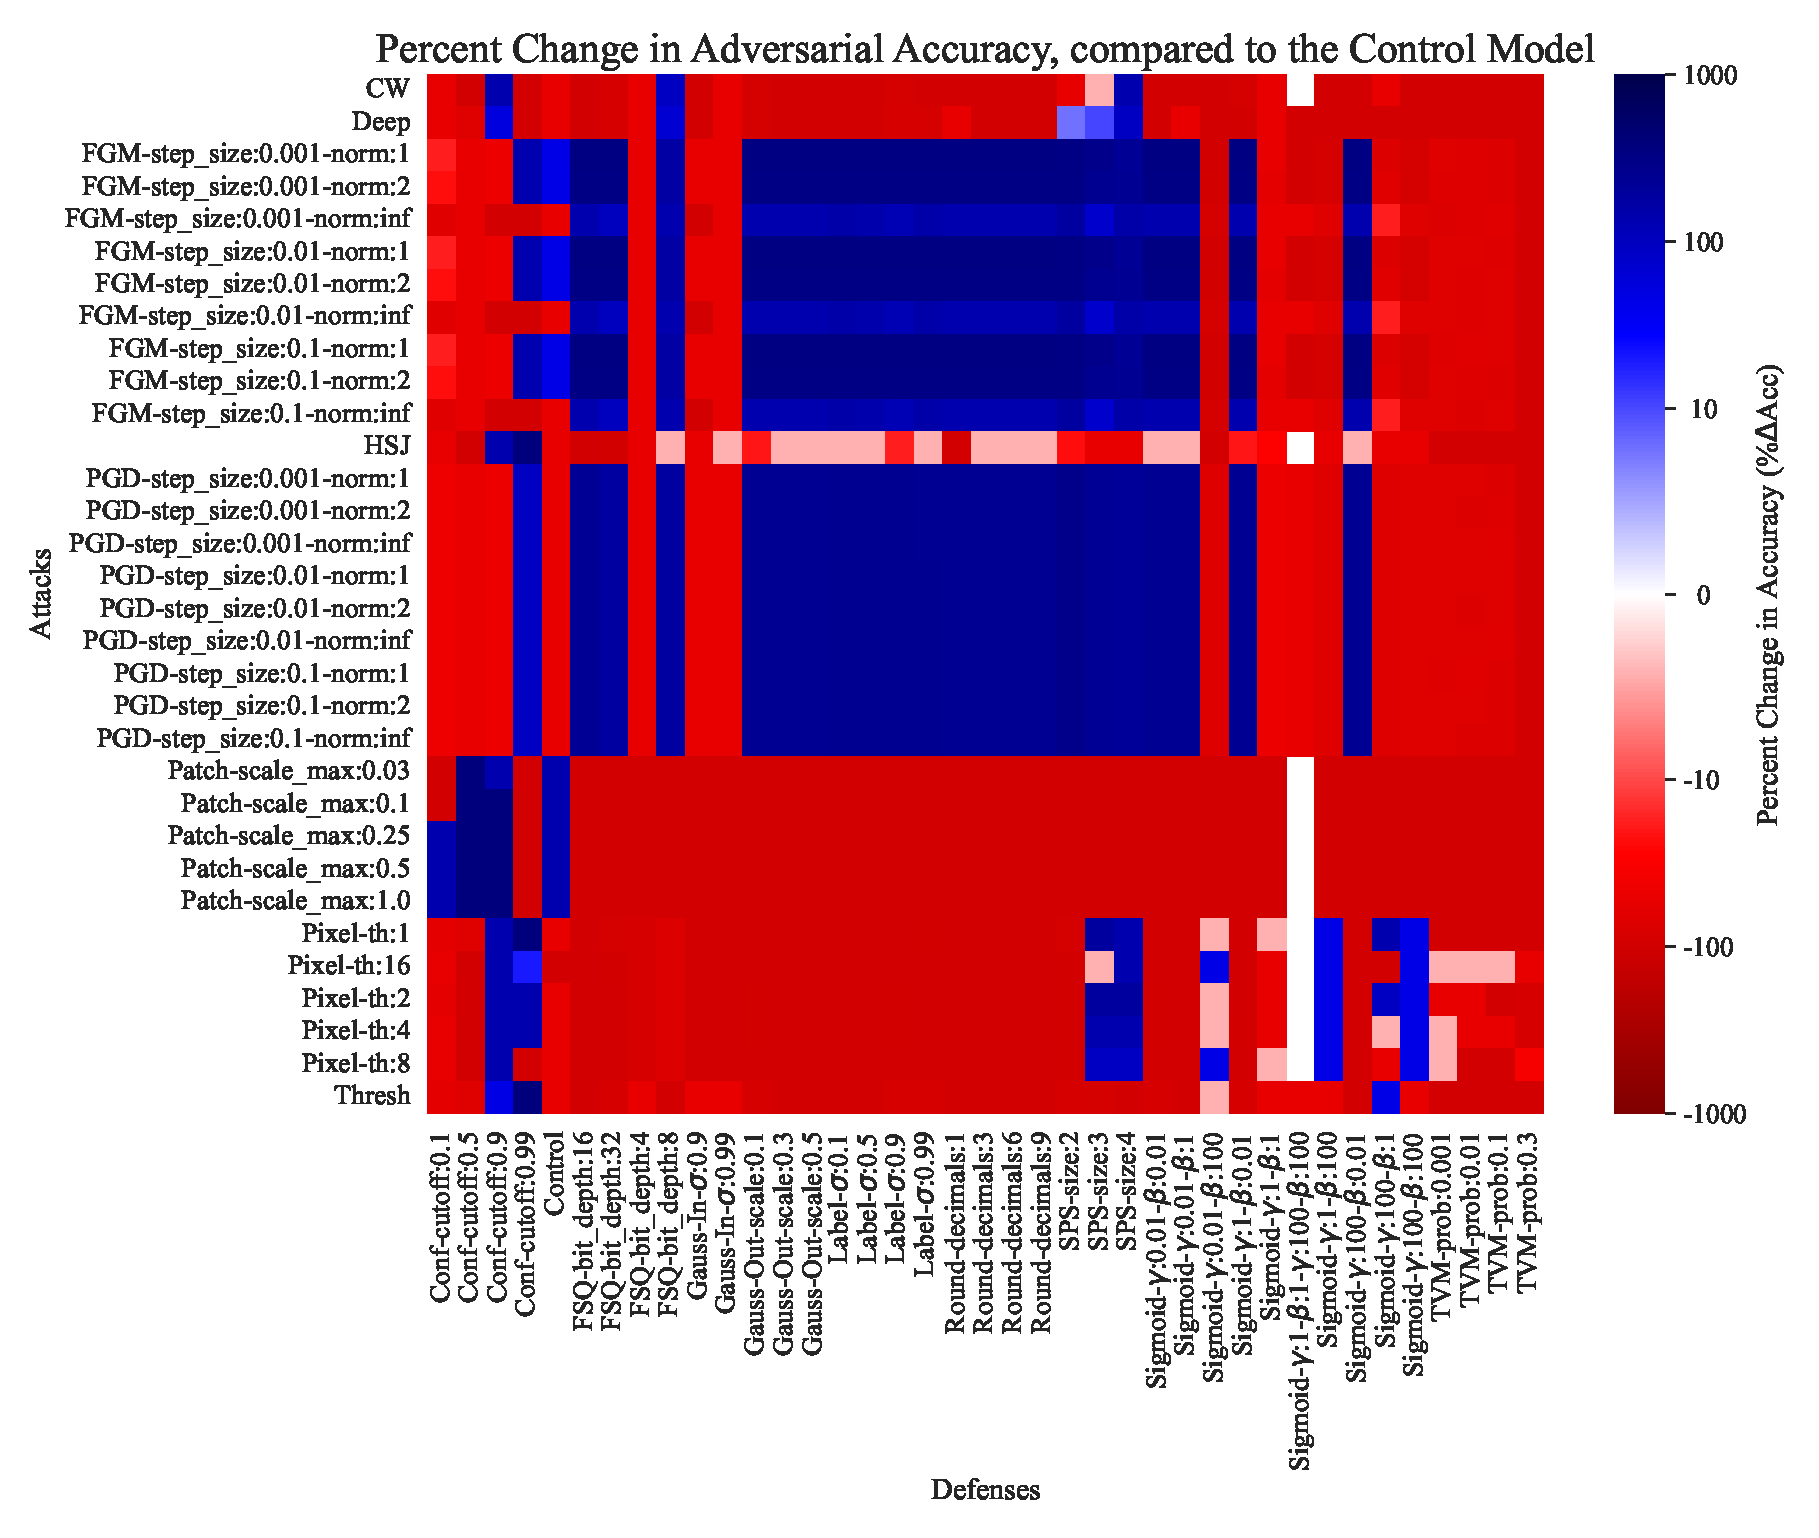
\includegraphics[trim={0 0.85em 0 0.4em},clip,width=0.7\textwidth]{Fig11.eps}
    \caption{The percent change in adversarial accuracy of each attack against each defense for CIFAR-10. As we can plainly see, no defense was able to improve the failure rate across all tested attacks. Red indicates that defense made a model worse. Blue indicates an improvement. White indicates no change.}
    \label{fig:adv_acc_grid}
    } % end centering
\end{figure*}

To generate confidence intervals, we varied both defense and attack parameters in an iterative grid search. Results across all tests are reported in Figures 4 and 8. Initial model weights and model architecture were taken from the survey by Madry et al \cite{madry2017towards}. Like in that paper (and commonly throughout the literature), we used the MNIST and CIFAR-10 datasets so that our survey can be directly compared to the wider literature. For each experiment, we trained the model for 20 epochs on the entire training set, as defined by the Tensorflow version of the datasets. Attacks were given a small computational budget of 10 iterations (100 samples, 10 iterations). For pre-processing defenses (see: Section \label{preprocessing}), this included data transformations that were distinct from the original training process and for post-processing defenses, the model output varied (see: Section V-B2) relative to the survey by Madry et al. \cite{madry2017towards}. The MNIST dataset was classified using a simple toy model and the CIFAR-10 dataset was classified using a modified  version of ResNet, both taken from the survey of Madry et al. \cite{madry2017towards}. Model prediction and attack times were measured using Python’s ‘process-time’ due to the timing jitter associated with shared systems and operating system variability. The timing resolution was in milliseconds, far below the scale of training times and total attack times, making
any noise negligible. After training, models were evaluated against the ten thousand unperturbed (benign) images available in the dataset according to both Equation 1 (accuracy) and
Equation 2 (failure rate) in both the benign context. Each model was attacked using the same subset of 100 (disjoint) samples, randomly drawn from this set in an attempt to isolate model performance from coincidences associated with sampling. Model accuracy on this set of perturbed data is denoted as the ‘adversarial accuracy’ below, with ‘benign accuracy’ referring to the model accuracy on the unperturbed data. All experiments were run on an Intel Xeon 4210 with 32GB of memory and with an Nvidia V100 GPU in a shared-kernel environment. We evaluated hundreds of combinations of attacks and defenses as illustrated and enumerated in Figure~\ref{fig:adv_acc_grid}.






\section{Results and Discussions}
\label{results}

\paragraph{Benign vs Adversarial Accuracy}

% % Accuracy across defenses and attacks
\begin{figure*}[!hptb]
    {\centering
    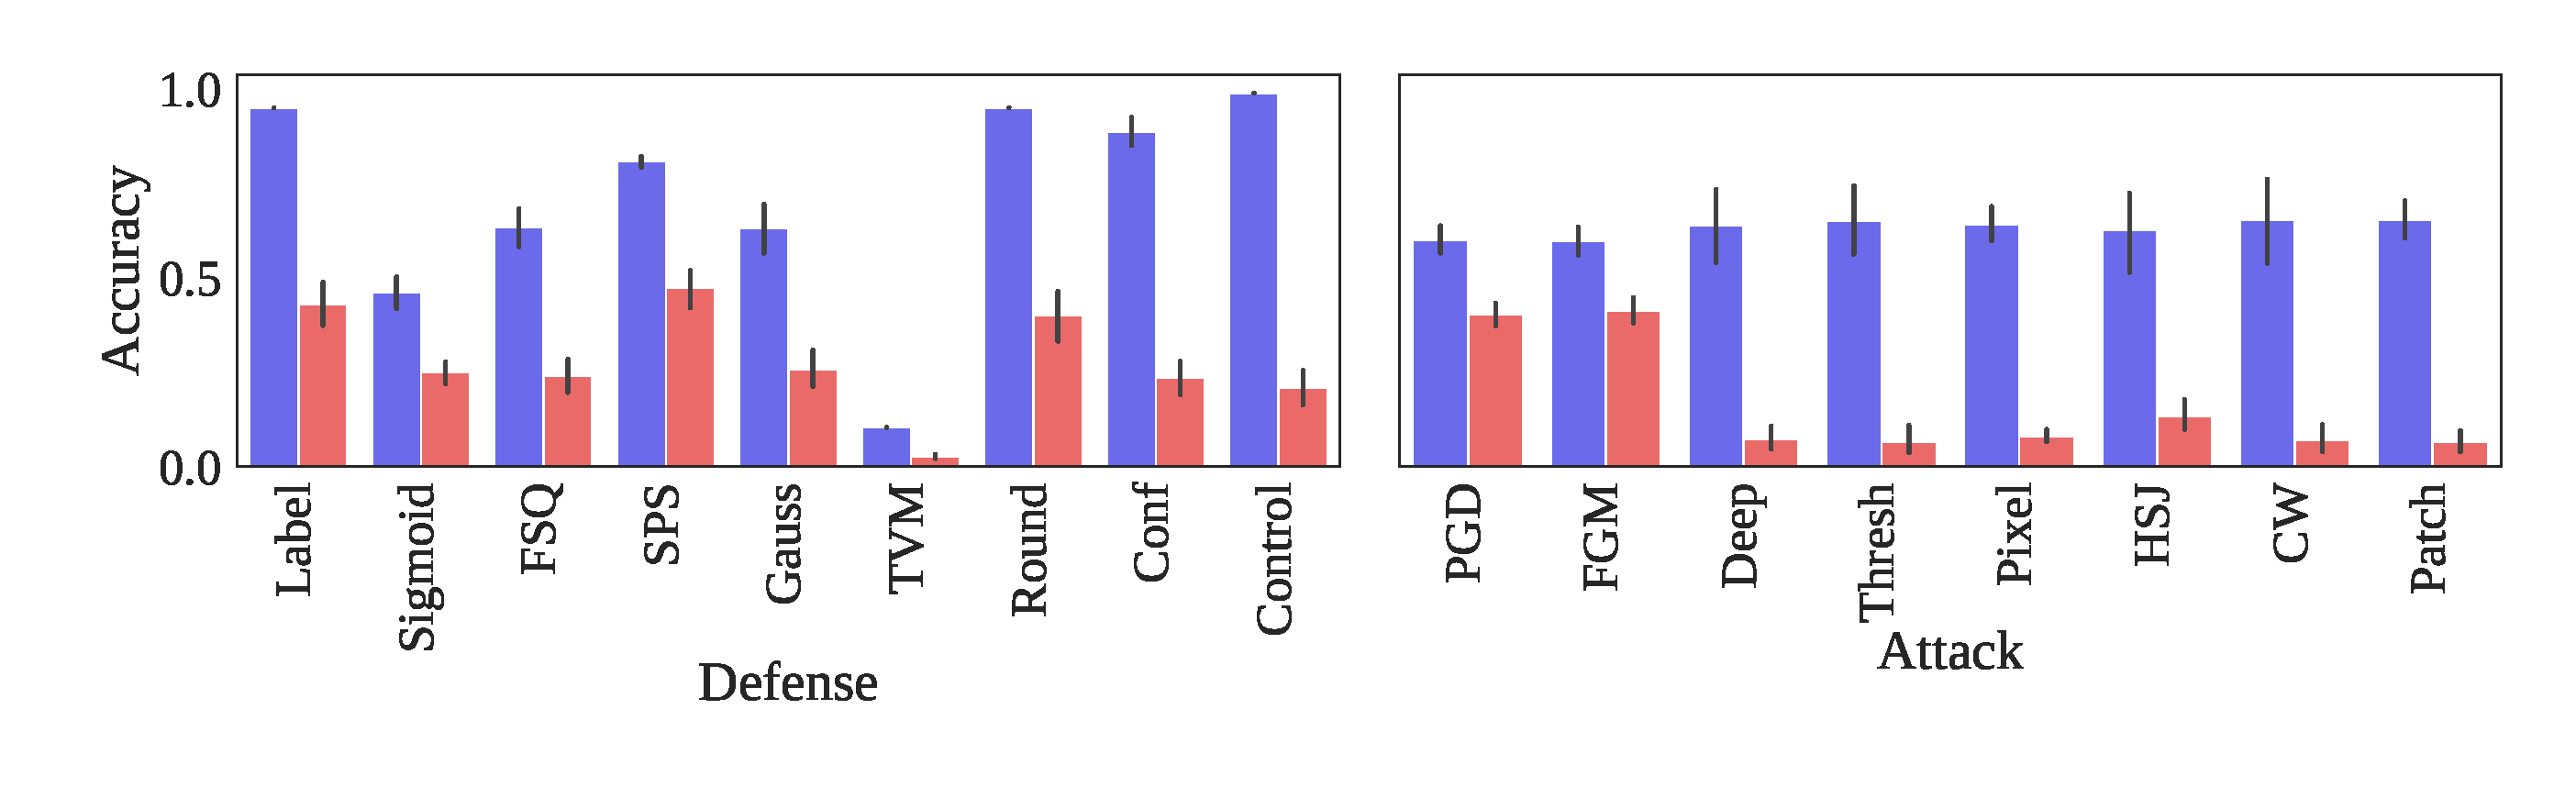
\includegraphics[trim={0 0.85em 0 0.4em},clip,width=0.9\textwidth]{Fig12.eps}
    \vspace{-1em}
    \caption{The 95\% confidence interval of adversarial (red) and benign (blue) accuracies for each defense (left) and each attack (right) for CIFAR-10. One trial was conducted for each hyper-parameter combination, and the confidence interval spans these trials.}
    \label{fig:acc}
    } % end centering
\end{figure*}

Figure~\ref{fig:acc} (left subplot) depicts the 95\% confidence region of adversarial and benign accuracy, computed using Equation~\ref{eq:accuracy}. The blue bars represent the accuracy on unperturbed (benign) data and the red bars represent the accuracy on perturbed (adversarial) data. From this rather large region (see Figure~\ref{fig:acc}), we see that both attack and defense hyper-parameter tuning have significant effects on the accuracy of a given method, since a small change in hyperparameters can drastically change the efficacy of a given attack or defense. Figure~\ref{fig:adv_acc_grid} shows the percent change in accuracy between the adversarial and benign circumstances for each defense and attack. We can plainly see that some techniques fool every model nearly every time while some attacks are weak and not likely to succeed under any conditions. Since no tested configuration reliably exceeded the \textit{benign accuracy}, this metric seems to only indicate a lower bound of the generalization error while the \textit{adversarial failure rate} estimates the upper bound (see Section~\ref{metrics}). That is, we can confidently claim that our \textit{true generalization error} ($\eta$) falls somewhere between $10^{-4}$ failures per second (roughly indicated by the 99.96 \% test-set, benign accuracy for MNIST or 99.83\% accuracy for CIFAR10) and the worst-case adversarial failure rate  (roughly $10^{-1}$ for MNIST and $10^{2}$ for CIFAR-10), which obviously falls below the safety-critical standards (see Table~\ref{tab:rate}) by huge margins, indicating that neither architecture is safety-critical (see: Section~\ref{safety-critical}).

\paragraph{Defenses}
    In Figure~\ref{fig:acc} we see that, for every defense (left subplot), that adversarial accuracy is lower than benign accuracy, adding more empirical evidence the accuracy \textit{vs.}~robustness trade-off discussed widely in the literature (\eg there robustness and accuracy are at odds with each other). The tested defenses each attempt to strategically destroy, smooth, or average data in the original dataset or the output of the model, which results in a loss of precision that makes the benign accuracy worse than the Control (see: Figure~\ref{fig:acc}). Furthermore, when we examine the attacks in the right subplot of Figure~\ref{fig:acc}, we see that Deep, HSJ, CW, Pixel, Patch, and Thresh are all able to confuse the model more that half of the time. Furthermore, variations in the defense performance (right side of Figures~\ref{fig:mnist_failure_rate}~and~\ref{fig:failure_rate}) raise questions about the ability of these architectures to generalize since things like bit-depth (FSQ), training-noise (Gausss-In), label-noise (Gauss-out), and image resolution (SPS) greatly vary the failure rate. In the real-world, effective resolution will change between individuals (e.g. a medical scan) or while moving (e.g. an autonomous vehicle). Even random noise drawn from approximately the same distribution as the training set (Gauss) increases the benign failure rate by an order of magnitude or two (compare the gap between \textit{Gauss} and \textit{Control} in both Fig.~\ref{fig:mnist_failure_rate} and Fig.~\ref{fig:failure_rate}). 
    
\paragraph{Attacks}
    Figure~\ref{fig:acc} (right subplot) depicts the same confidence region as above, but broken down by attack rather than defense. It is obvious that the Deep, HSJ, and Patch reduce the accuracy the most often. PGD, FGM, and CW are less effective, but still able to successfully perturb a significant portion of the samples. However, the Threshold and Pixel attacks are less consistent.Figure~\ref{fig:adv_acc_grid} demonstrates how each attack fares against each defense by depicting the percent change in accuracy. The color gradient is centered at the benign failure rate, becoming a more intense red as the accuracy decreases, with a dark red indicating substantially worse performance than with the undefended model and unperturbed data. Since no column is blue in Figure~\ref{fig:adv_acc_grid}, no single defense is able to consistently subvert a generalized attacker, while modest gains against a particular attack are possible. Techniques like Adversarial Patch, DeepFool, and HopSkipJump consistently break models (see: Figure~\ref{fig:adv_acc_grid}). While some defenses do provide limited protection against more advanced techniques (indicated by the color blue in Figure~\ref{fig:adv_acc_grid}), their performance on unperturbed data tends to be reduced relative to the control (see: Figure~\ref{fig:acc}, left subplot) substantial empirical evidence that the normally discussed accuracy, from Equation~\ref{eq:accuracy}, is consistently more optimistic than what the adversarial analysis implies.

%% Fit and pred time across defenses and attacks
\begin{figure*}[!hptb]
    {\centering
    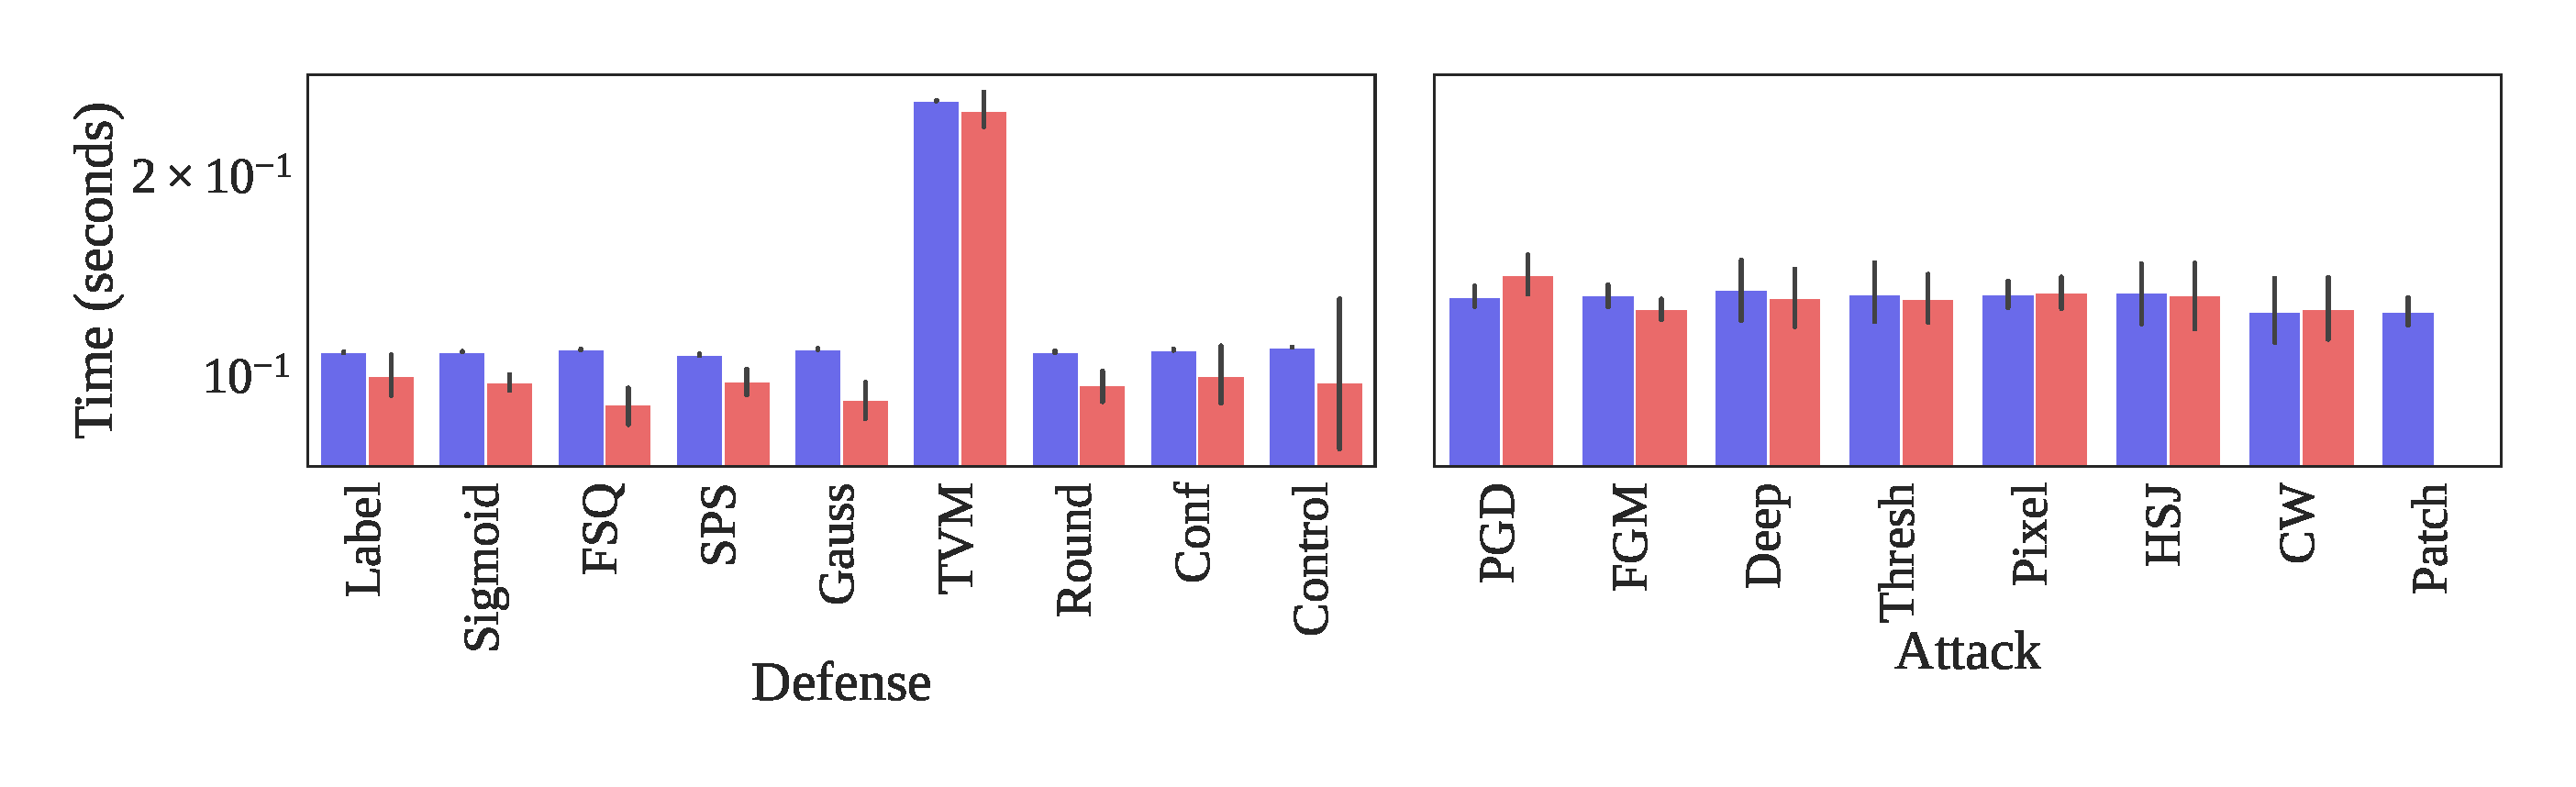
\includegraphics[trim={0 0.85em 0 0.35em},clip,width=0.9\textwidth]{Fig13.eps}
    \vspace{-1em}
    \caption{The 95\% confidence interval of prediction times (blue) and attack times (red) for CIFAR-10, broken down by defense (left) and attack (right). One trial is depicted for each hyper-parameter combination. Accuracy on the benign (unperturbed) dataset is depicted in blue and accuracy on the adversarial (perturbed) dataset is depicted in red.}
    \label{fig:time}
    } % end centering
\end{figure*}

\begin{figure*}[!hptb]
    {\centering
    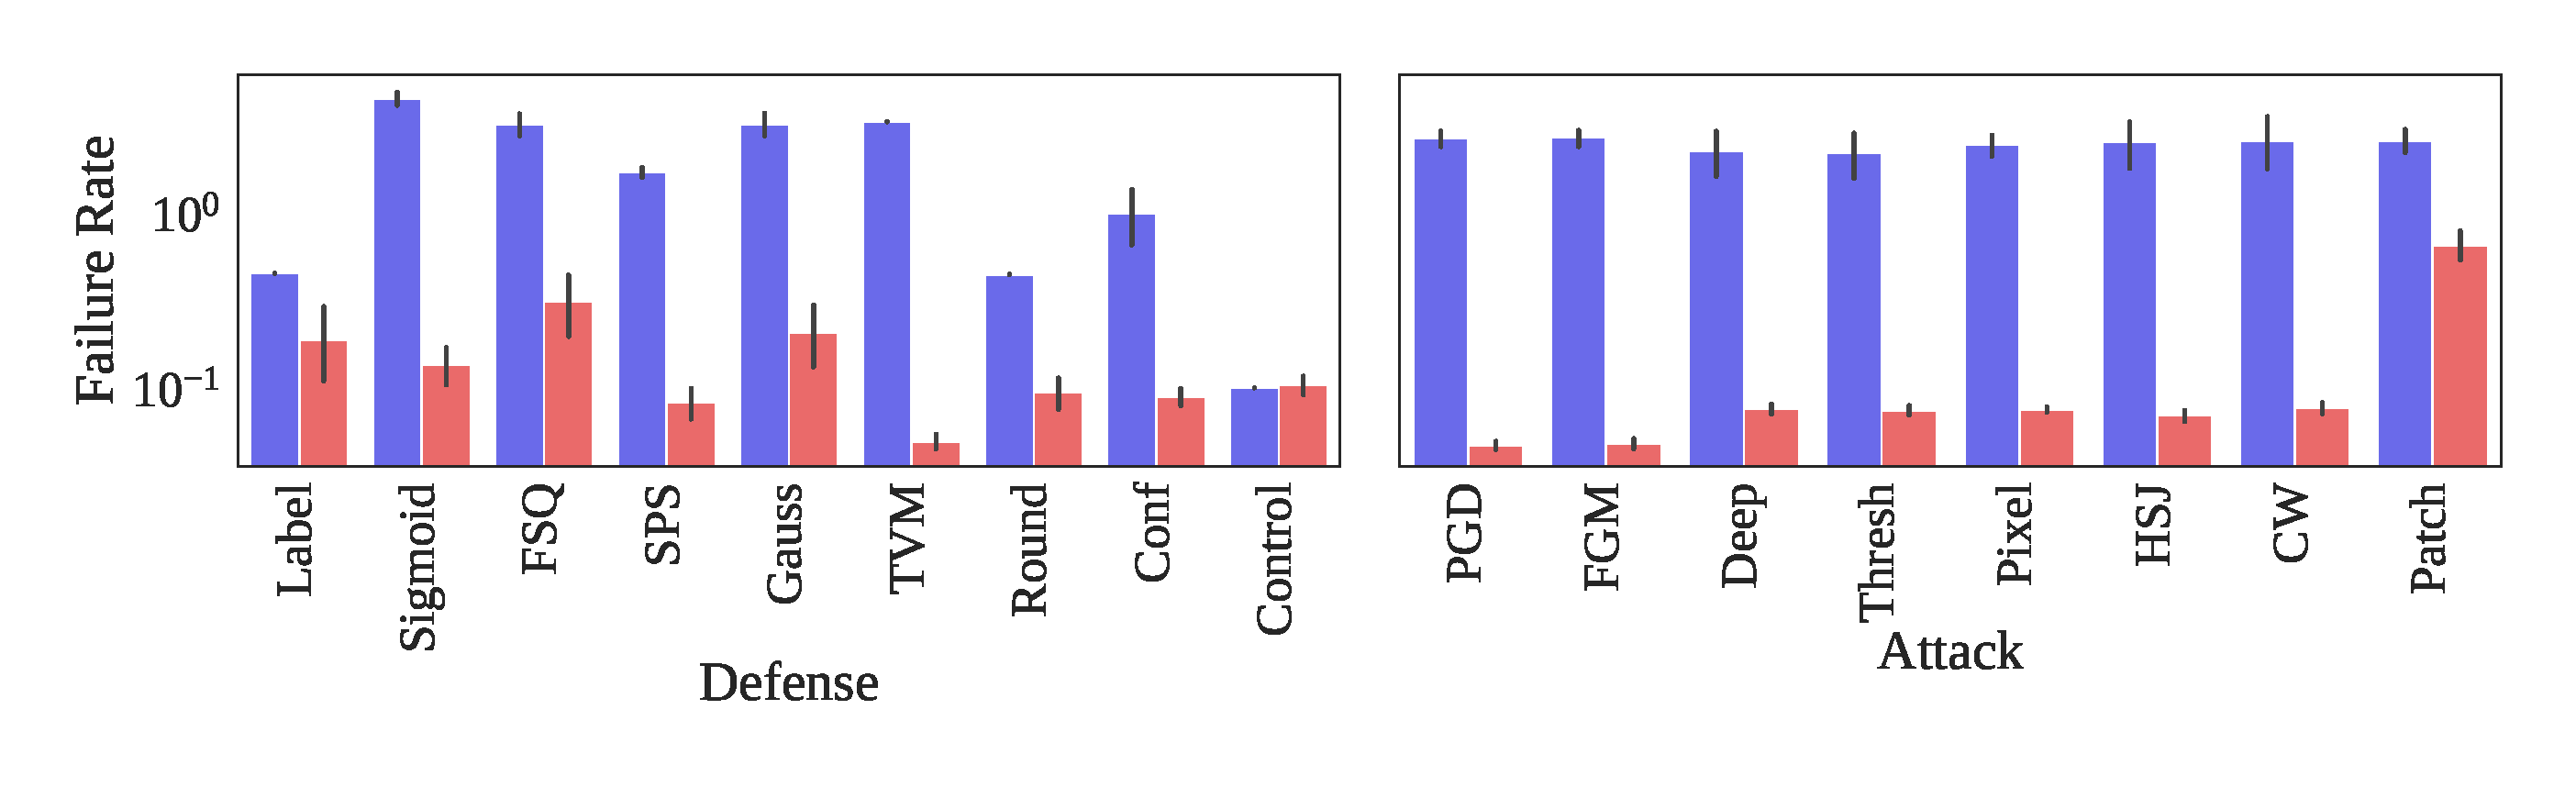
\includegraphics[width=0.9\textwidth]{Fig14.eps}
    \vspace{-1em}
    \caption{The 95\% confidence interval of failure rates both benign (blue) and adversarial (red) for CIFAR-10, broken down by defense (left) and attack (right). This was computed using Equation~\ref{eq:failure_rate}. The failure rate of the benign (unperturbed) dataset is depicted in blue and the failure rate of the adversarial (perturbed) dataset is depicted in red.}
    \label{fig:failure_rate}
    } % end centering
\end{figure*}

\paragraph{Computational Cost}

 In order to estimate computational cost, we measured each time as a process time, reducing the jitter due to operating system operations and shared kernel constraints. We see that defenses require between 1 and 100 seconds of training per success, broken down by defense in the left subplot of Figure~\ref{fig:time}. However, attacks (see right subplot of Figure~\ref{fig:time}) require as few as several milliseconds per sample in the worst case and $10$ seconds in the best case, with the average attack time falling after around a half second per sample. Furthermore, we see that the  Figure~\ref{fig:failure_rate}, we see how various defenses manage the trade-off between computational complexity and efficacy by measuring the failure rate as in Equation~\ref{eq:failure_rate}. The Confident model had the best accuracy (see: Figure~\ref{fig:acc}) since it merely ignores queries below a certain confidence threshold, but even if we treat that as a null event (instead of a false classification), this increases the failure rate (see: Figure~\ref{fig:failure_rate}) relative to the control since objects were not detected.
 

\paragraph{Failure Rate}

When we combine the information from the accuracy and time graphs in Equation~\ref{eq:failure_rate}, we obtain Figure~\ref{fig:rate_grid}, displaying the failure rate across attacks and defenses as well as their individualized performance.  
%% Rate
\begin{figure*}[!hptb]
    {\centering
    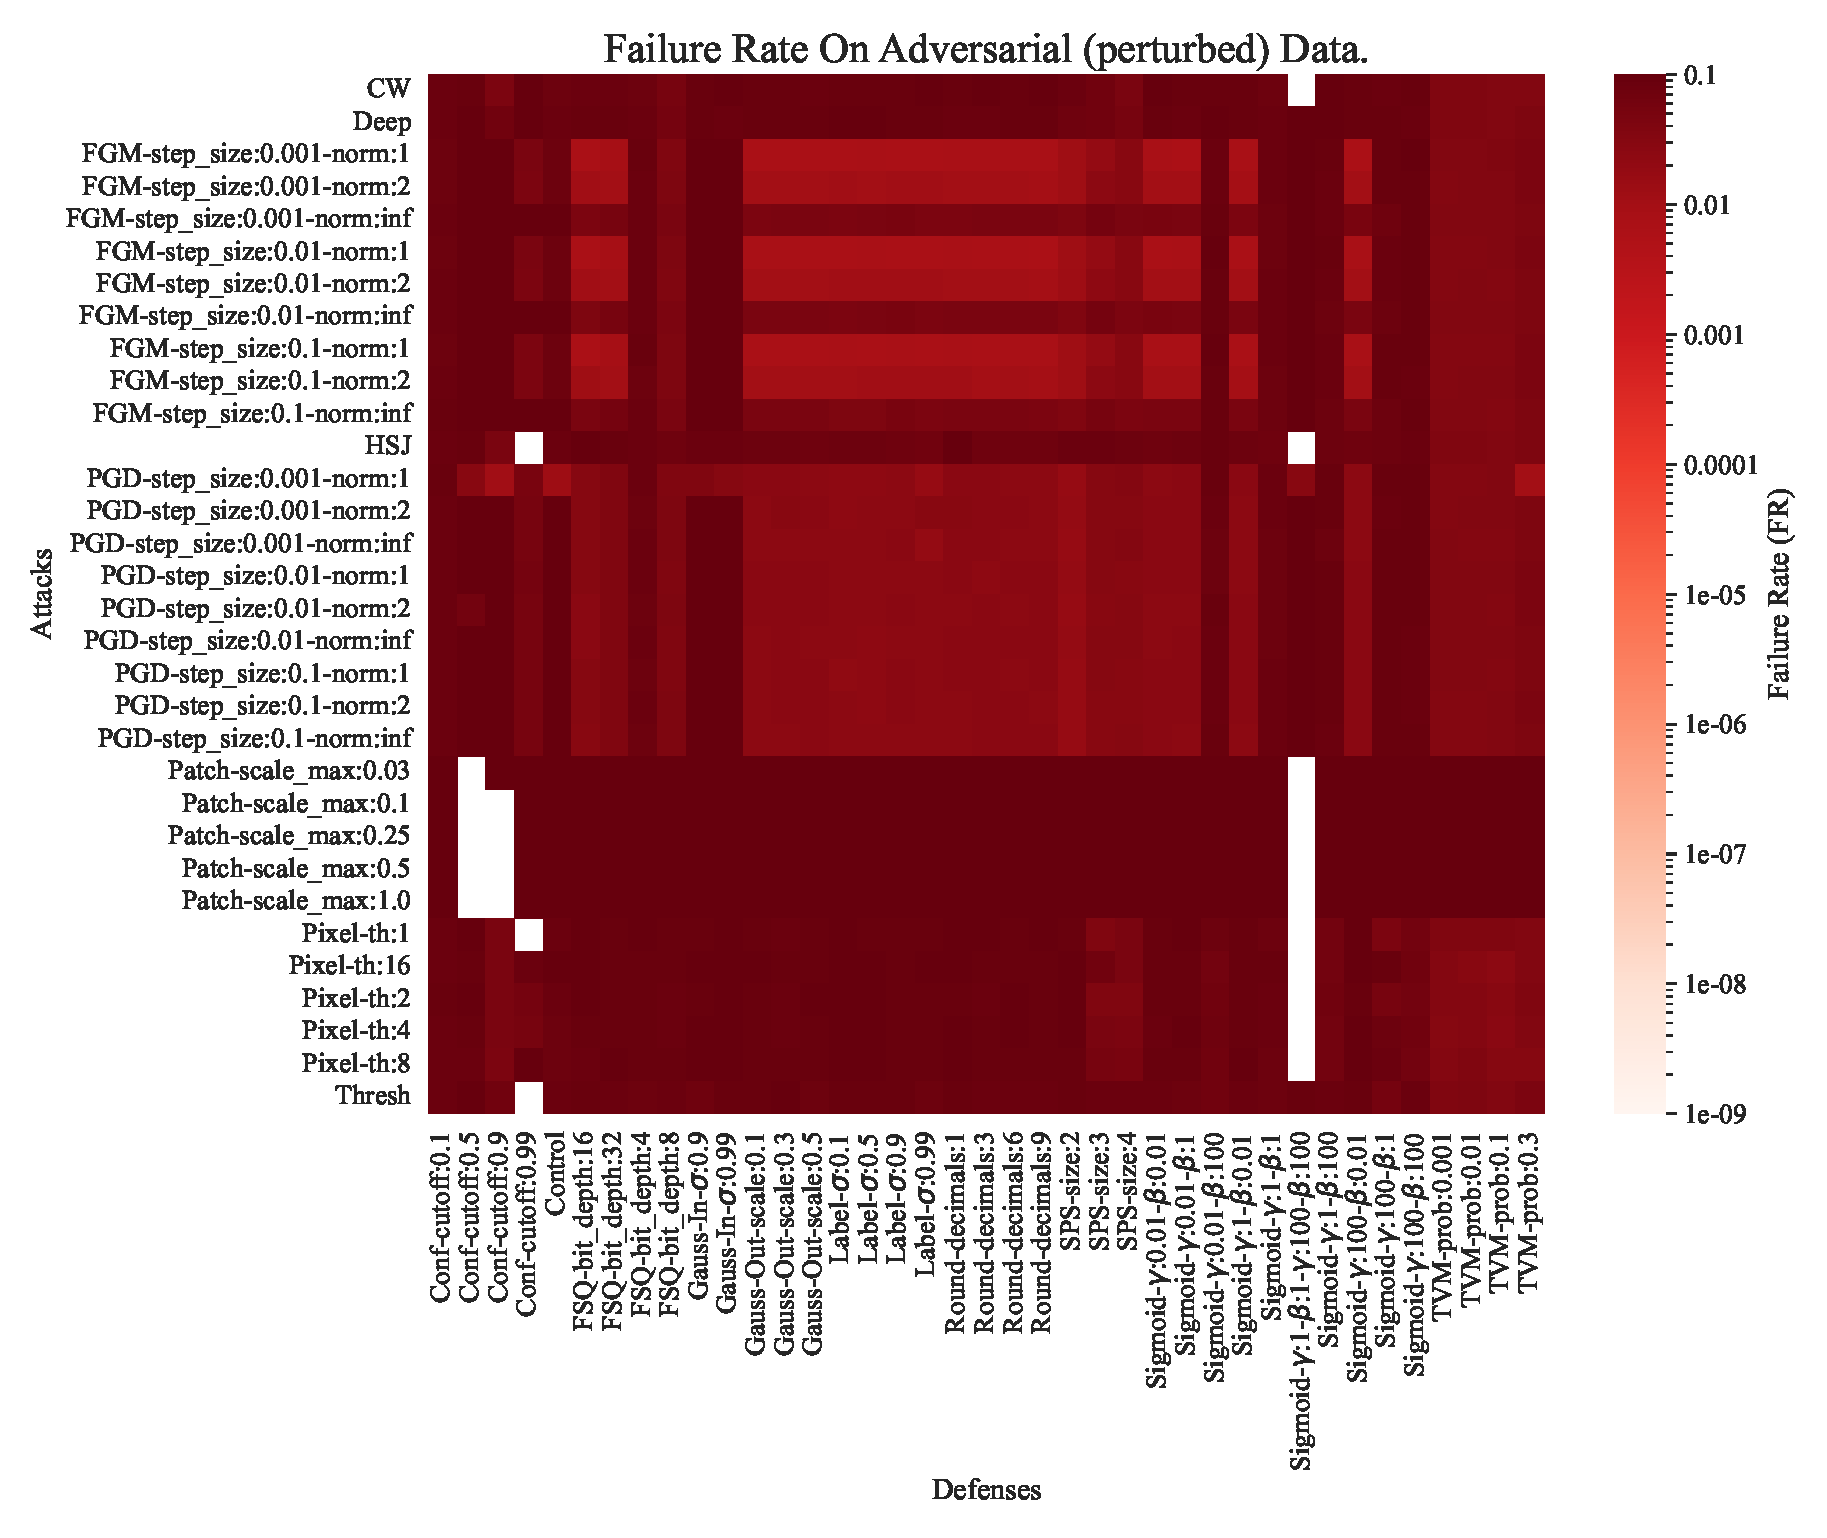
\includegraphics[trim={0 0.85em 0 0.35em},clip,height=0.6\textwidth]{Fig15.eps}
    \vspace{-0.75em}
    \caption{The adversarial failure rate for all attacks and defenses for CIFAR-10. Darker red means worse performance and white indicates that no adversarial \cm{samples} were found. This result is rather pessimistic, suggesting that all configurations fail to meet industrial standards.}
    \label{fig:rate_grid}
    } % end centering
\end{figure*}
When we examine the average performance of a given defense (see: Figure~\ref{fig:rate_grid}), we see that most defenses fail to meet safety critical standards (see: Table~\ref{tab:rate}), even if the surveyed defenses tend to improve adversarial accuracy (see: Figure~\ref{fig:change_grid}). Total Variance Minimization produced particularly inaccurate models which led to particularly inaccurate attacks.  While some defenses do provide relief against some attacks, that behavior is inconsistent across different attacks, particularly in the case of the Patch and Pixel attacks which seem to be universally strong, even with mild perturbation constraints. Furthermore, those gains are marginal compared to the efficacy of the average attack (see: Figure~\ref{fig:change_grid}) and the order of magnitude required by regulations (see: Figure~\ref{tab:rate}).
%% Failure rate across defenses and attacks


\paragraph{Attack Budget and Attacker Knowledge}
When we examine the general performance characteristics of attacks, we see that the average attack takes a few seconds to induce a failure (see Figures~\ref{fig:mnist_failure_rate}~and~\ref{fig:failure_rate}). This appears to be consistent across attacks and is remarkably effective with only a small computational budget of 100 iterations and a query budget of 1000 with a perturbation distance no greater than 1 byte. This is true for both whitebox attacks  (everything but HSJ) and blackbox (HSJ) attacks. Most attacks take a few seconds per sample; however, the one exception to this is the Adversarial Patch attack which takes only a few milliseconds to induce a failure (on average). Due to the universality of this attack against an entire dataset (see Section~\ref{attacks}) this failure rate would go to infinity as the sample size goes to infinity. In practice, a quadratic approximation of the boundary (HSJ) is roughly as effective as whitebox models, especially as the number of features scale (compare Figure~\ref{fig:mnist_adv_acc_grid}~and~Figure~\ref{fig:adv_acc_grid}). However, there is a clear advantage when the attacker optimizes across a large sample of the test set (see \textit{Patch} in Section~\ref{attacks}), with the failure rate tending towards 0 as this sample size increases. Furthermore, by simulating a black-box attack (HSJ attack), regularizing generated examples for false confidence (CW attack), finding minimal separating planes (Deep attack),  and using advanced optimization techniques to generate highly confident false examples (Thresh attack), we were able to consistently fool the models in mere milliseconds per sample. The simplest attacks, which Madry et al.~proposed in 2017, remain effective (PGD, FGM). Furthermore, proper step-size tuning seems to compensate for this simplicity. This is evidenced by right side of Figures~\ref{fig:mnist_failure_rate}~and~\ref{fig:failure_rate}, suggesting that the gradient ascent attacks might be a `good enough' estimator of the generalized failure rate, especially given the astronomical gap between current test-set accuracy and regulatory requirements.


\paragraph{Percent Change in Accuracy}

Figure~\ref{fig:adv_acc_grid} demonstrates how each attack fares against each defense. The color gradient starts at white, indicating the undefended model's performance against unperturbed data, becoming a more intense red as the accuracy decreases, with blue indicating an increase in accuracy compared to the control model. As we can plainly see, no single defense is able to consistently subvert an attacker.  While some defenses do provide limited protection against more advanced techniques, their performance against gradient descent techniques is inconsistent at best. Furthermore, for DeepFool and HopSkipJump, we know that they could lead to even worse results for the defender, given a larger computational budget. While there is limited efficacy against gradient-based attacks for some defenses, advanced techniques like Adversarial Patch, DeepFool, and HopSkipJump consistently break models. That is, we provide substantial empirical evidence that the normally discussed accuracy from Equation~\ref{eq:accuracy} is, at best, an optimistic estimate of the real-world failure rate.



\paragraph{Percent Change in Failure Rate}
%% Change Grid
\begin{figure*}[!hptb]
    {\centering
    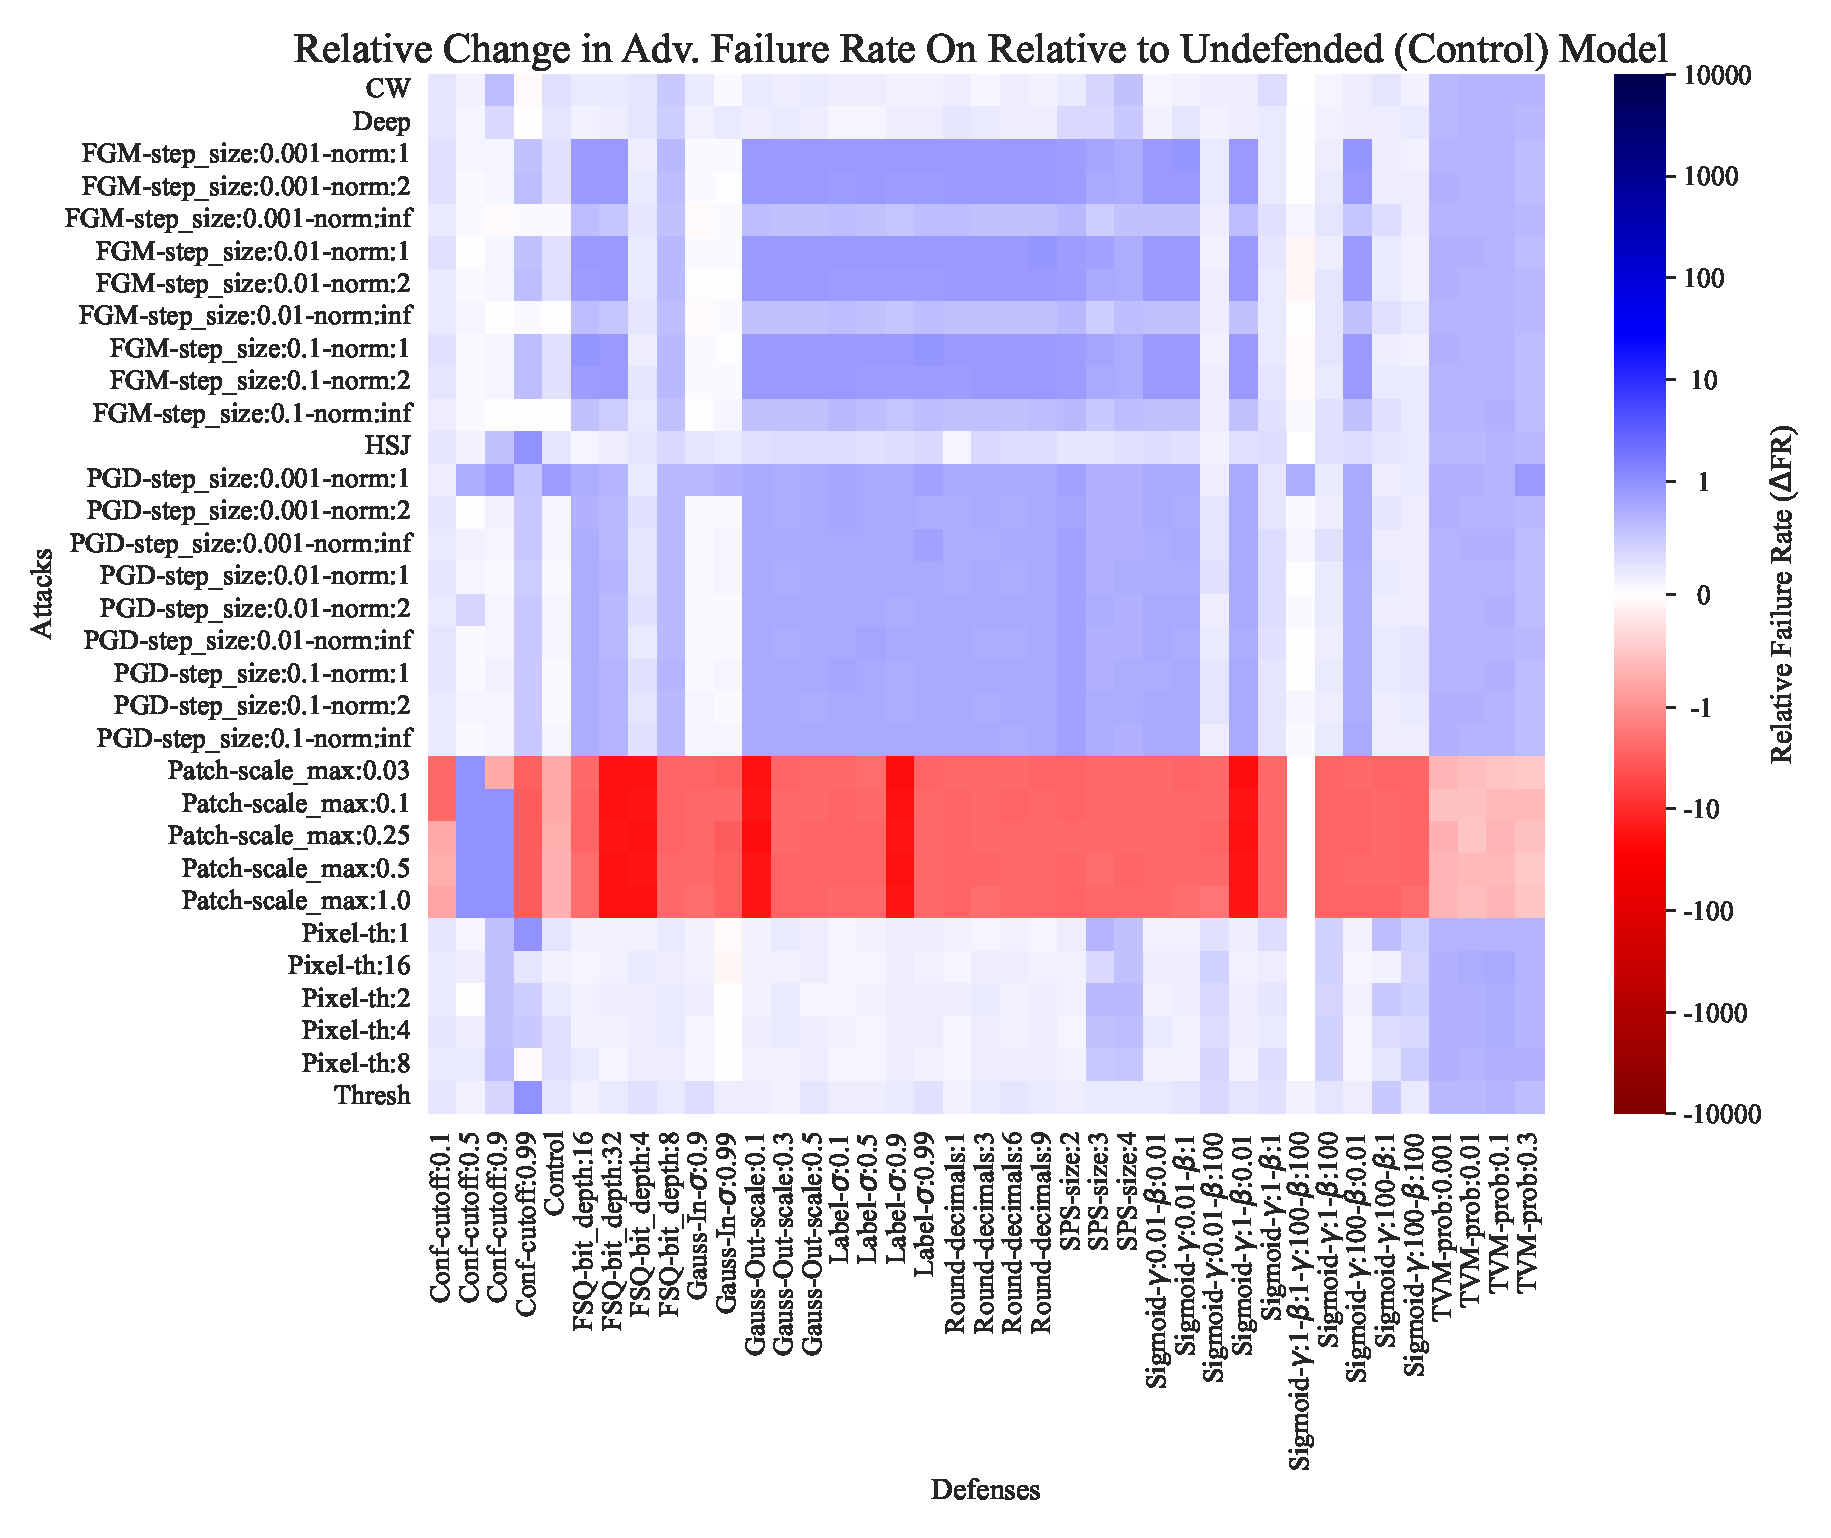
\includegraphics[trim={0 0.85em 0 0.35em},clip,height=0.6\textwidth]{Fig16.eps}
    \vspace{-0.75em}
    \caption{The relative change in failure rate for the adversarial case, centered at the benign failure rate for CIFAR-10. Blue indicates an improvement relative to the benign (unperturbed) case. Red indicates a worsening of performance in the adversarial case compared to the benign case. White indicates no change. Note that the scale is logarithmic so that marginal gains and substantial losses can be seen clearly.}
    \label{fig:change_grid}
    } % end centering
\end{figure*}


% % Accuracy across defenses and attacks
\begin{figure*}[!htbp]
    {\centering
    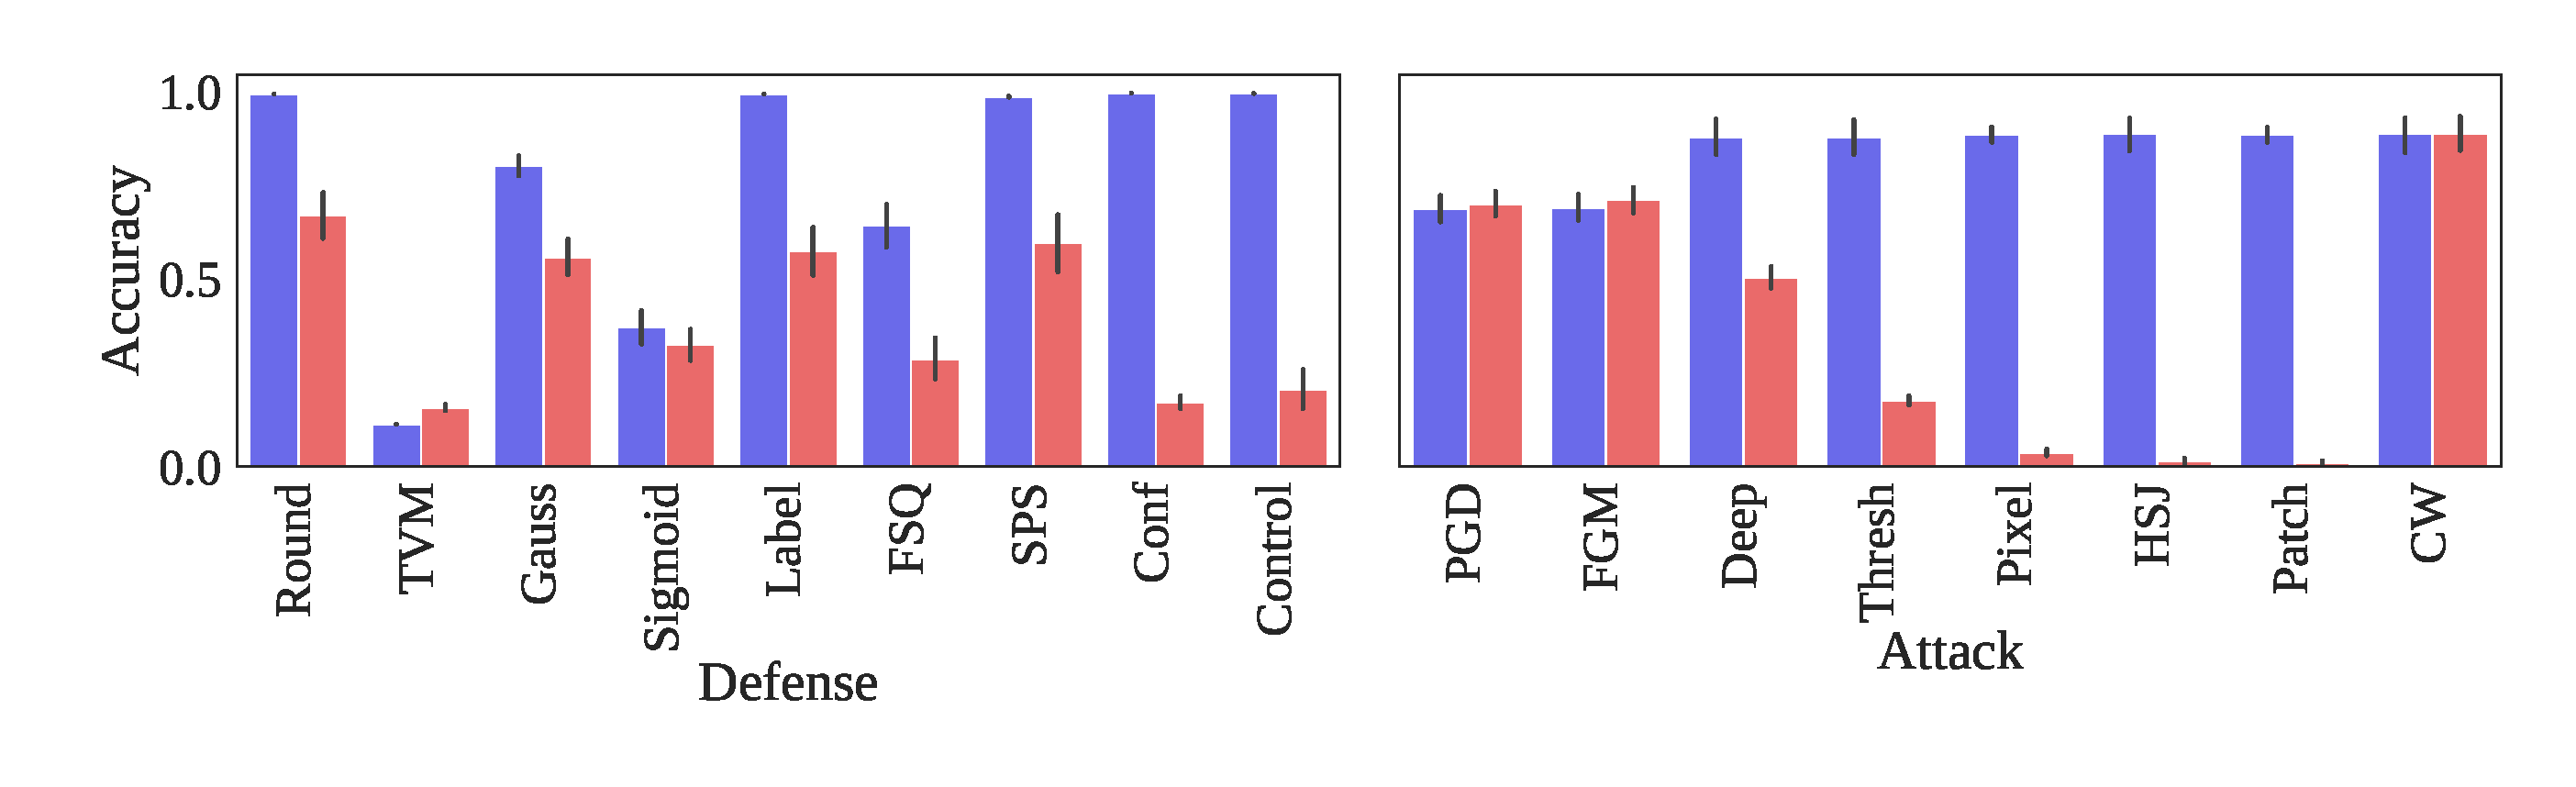
\includegraphics[trim={0 0.85em 0 0.5em},clip,width=0.9\textwidth]{Fig17.eps}
    \vspace{-1em}
    \caption{The 95\% confidence interval of adversarial and benign accuracies for each defense (left) and each attack (right) on the MNIST dataset, broken down by defense (left) and attack (right). One trial was conducted for each hyper-parameter combination.}
    \label{fig:mnist_acc}
    } % end centering
\end{figure*}



%% Adv Accuracy Grid
\begin{figure*}[!htbp]
    {\centering
    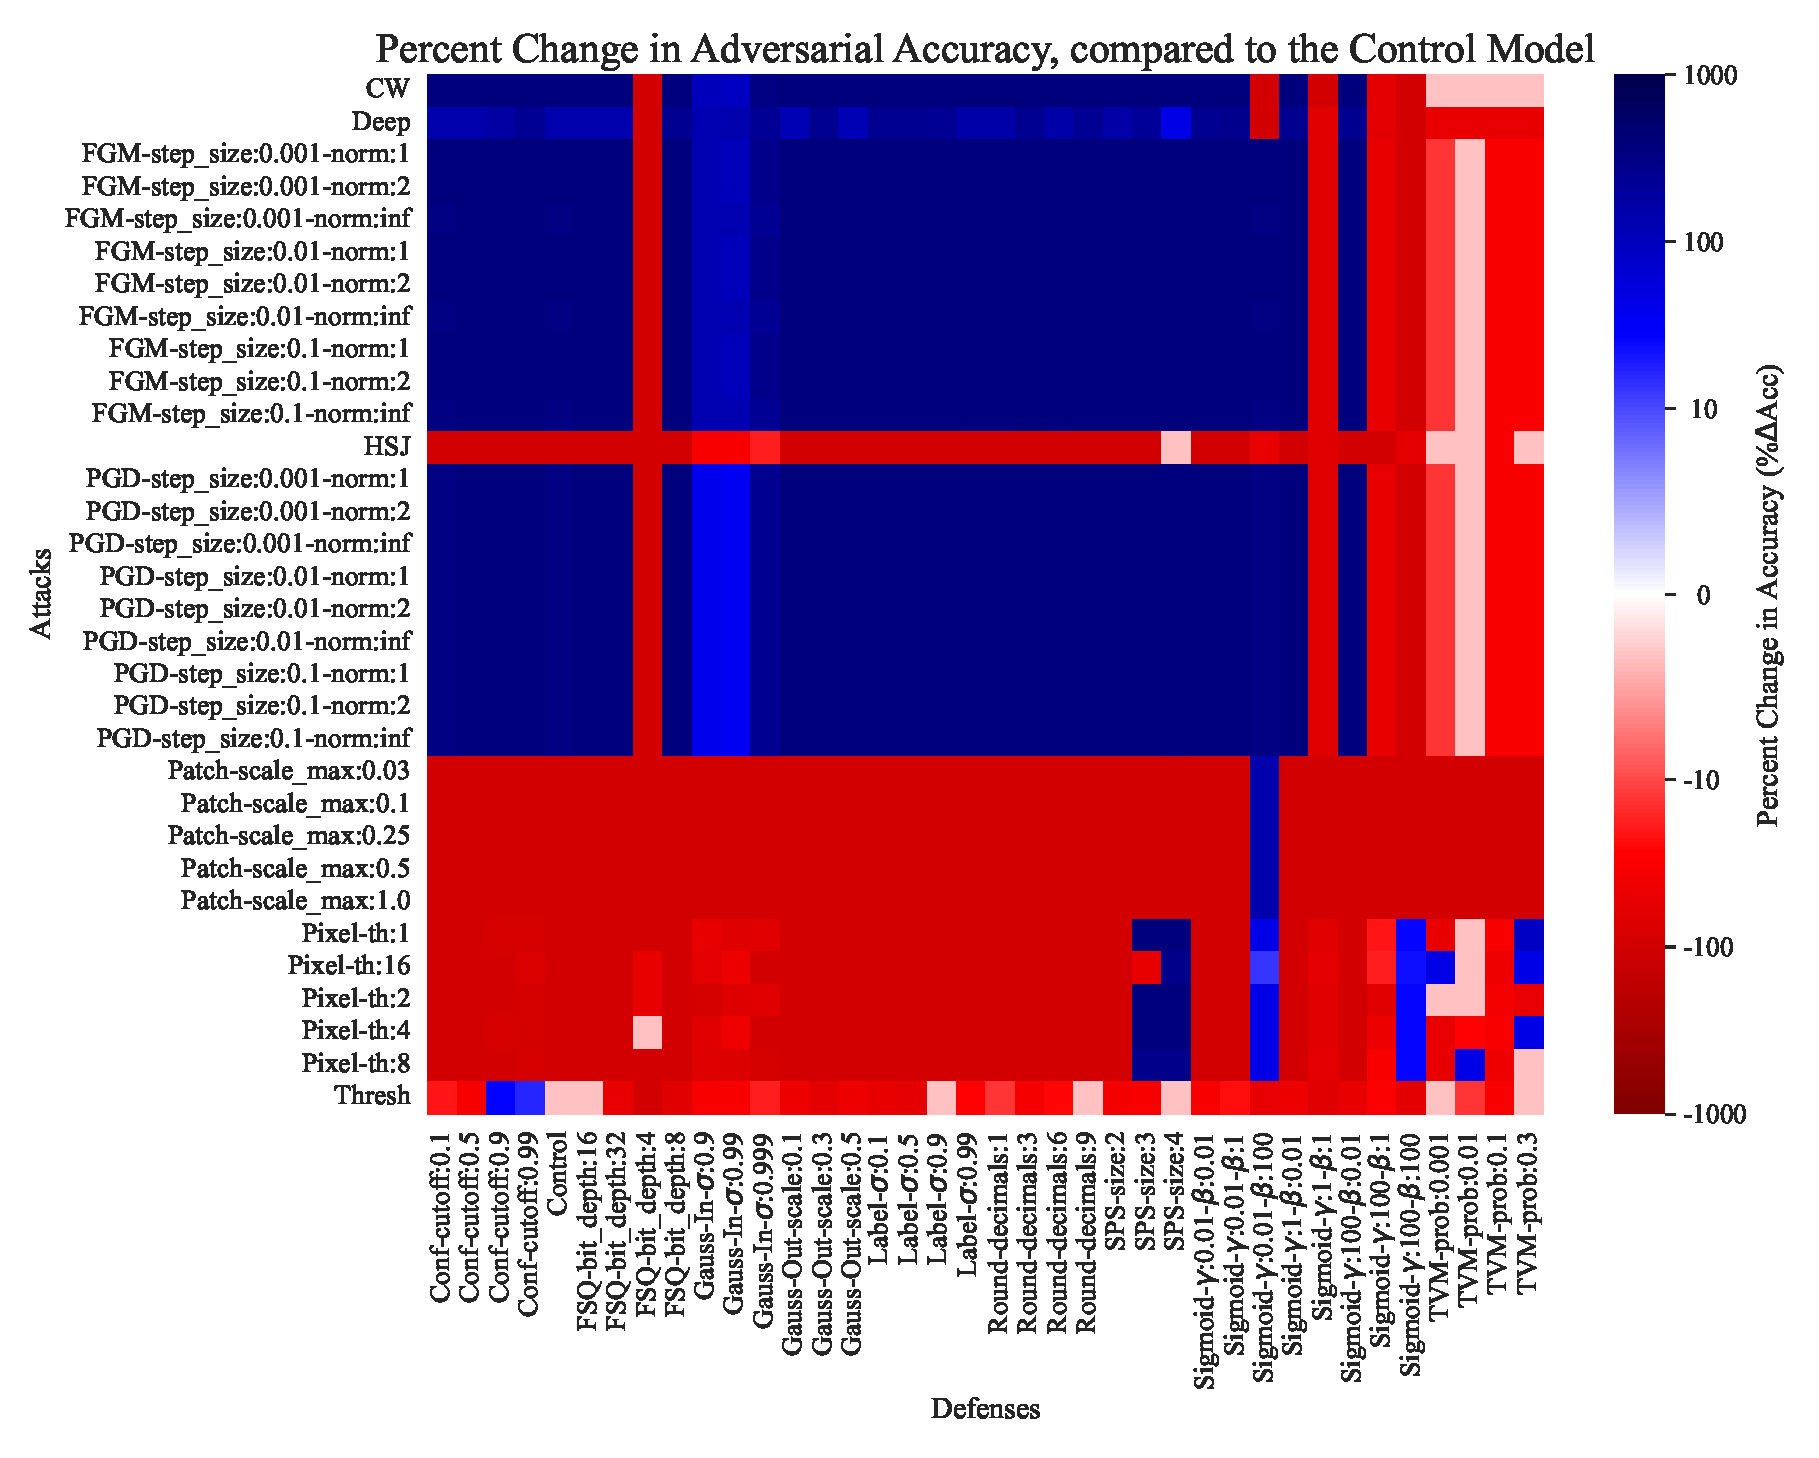
\includegraphics[trim={0 0.85em 0 0.35em},clip,height=0.58\textwidth]{Fig18.eps}
    \vspace{-0.5em}
    \caption{The adversarial accuracy of each attack against each defense on the MNIST dataset. Blue would indicate an improvement relative to the undefended model. Red indicates that defense made a model worse. White indicates no change. This was computed using Equation~\ref{eq:percent_change_acc}.}
    \label{fig:mnist_adv_acc_grid}
    } % end centering
\end{figure*}


Figure~\ref{fig:change_grid} depicts how each defense fares against each attack by comparing the change in failure rate when compared to the adversarial case on the undefended model. When we compare this plot to the one in Figure~\ref{fig:adv_acc_grid}, we see that, in many cases, the defenses were able to decrease the adversarial failure rate when compared to the undefended model, which is what these defenses intended to do. However, increased safety (depicted as blue in Figure~\ref{fig:change_grid}) is marginal at best---on the order of a few percent (see: Figure~\ref{eq:relative_change_failure_rate}) when measured rates are many orders of magnitude from regulatory standards (see: Table~\ref{tab:rate}). Additionally, the potential downsides of a given defense are much larger (see: Figure~\ref{fig:adv_acc_grid}). This marginal improvement in the failure rate is driven largely by the marginal time cost (see: Figure~\ref{fig:time}) rather than the accuracy (see: Figure~\ref{fig:acc}). That is, the defenses increase the adversarial accuracy, but also take significantly longer (see: Figure~\ref{fig:time}).


\paragraph{MNIST \textit{vs.}~CIFAR-10}
In addition to running these experiments on the CIFAR-10 dataset, we also ran them on the MNIST dataset using a simpler model provided by Madry \textit{et al.}~\cite{madry2017towards}. Figure~\ref{fig:mnist_acc} broadly verifies the behavior observed above on the CIFAR-10, wherein defenses tend to reduce model accuracy on the benign set, gradient-based attack efficacy is largely determined by hyperparameter tuning, and non-gradient-based attacks are still very effective. As with CIFAR-10, no defense was able to improve the benign (unperturbed) accuracy of the undefended model for every attack (see: Figure~\ref{fig:mnist_adv_acc_grid}). Despite a smaller model and lower run-time requirements (compare Figure~\ref{fig:mnist_time} to Figure~\ref{fig:time}), we see that training time is more-or-less the same. When we compare Figure \ref{fig:rate_grid} with Figure \ref{fig:mnist_rate_grid}, we see that some of the defenses were much more effective at preventing gradient-descent attacks. However, they failed against the more computational expensive techniques of Patch, HSJ, and Deep. Then, when we examine failure rate (Figure~\ref{fig:mnist_failure_rate}), we see that despite being a different dataset and model architecture, we are still able to induce failures in only a few seconds, as with CIFAR-10. However, when we break this rate down into each attack and defense combination and measure a change in the failure rate (see: Figure~\ref{fig:mnist_change_grid}), there seems to be a fairly consistent and marginal improvement driven by time (see: Figure~\ref{fig:mnist_time}) rather than accuracy (see:  Figure~\ref{fig:mnist_acc}), as with CIFAR-10. When we applied defenses to the simpler MNIST model and dataset (when compared to CIFAR-10), we found largely consistent results. However, we did find that there were more cases of failed adversarial attacks against MNIST, likely due to the significantly smaller dimensionality of both the dataset and model~\cite{dohmatob_generalized_2019}. However, we would expect real-world data to be significantly higher resolution and full-color, unlike the black and white low-resolution images typical of MNIST, so those results probably underestimate the severity of the problem in real-world systems that use multiple multi-pixel RGB cameras to classify objects in real-time. 


 %% Fit and pred time across defenses and attacks
\begin{figure*}[!hptb]
    {\centering
    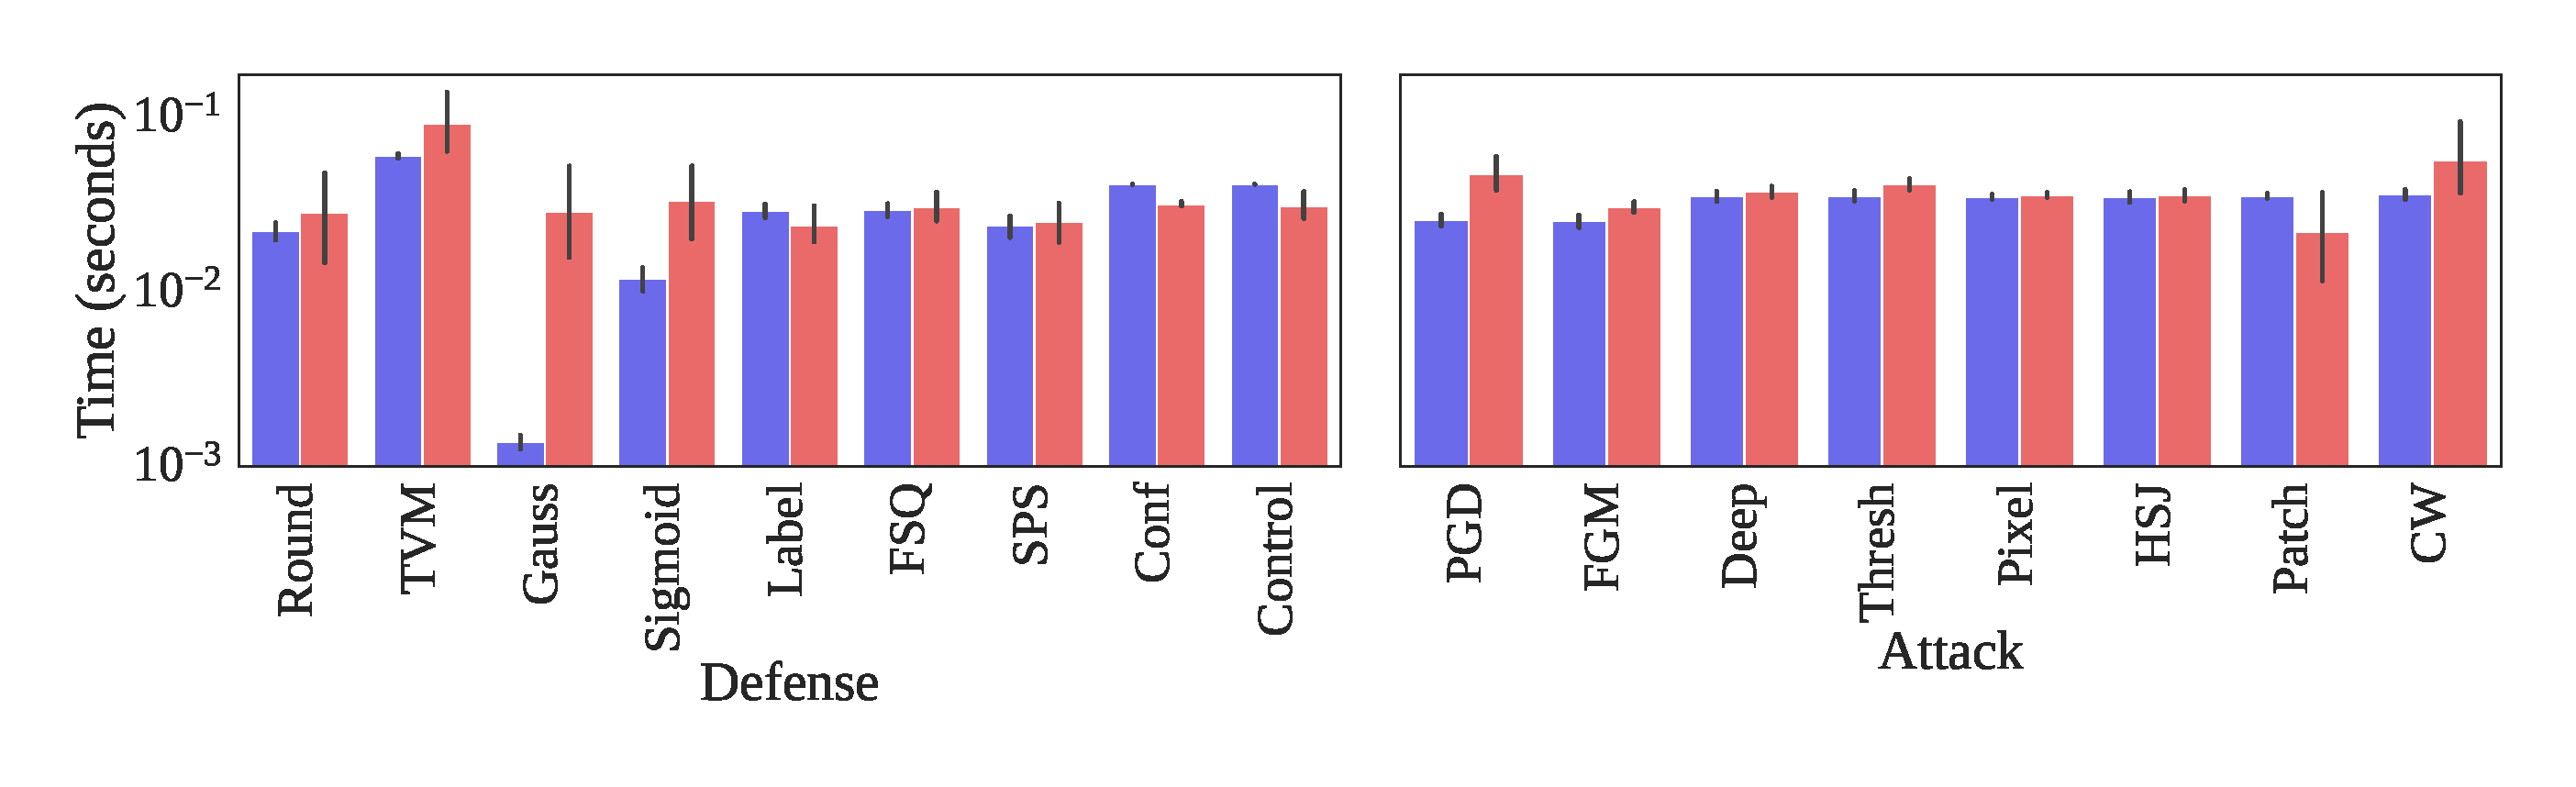
\includegraphics[trim={0 0.85em 0 0.35em},clip,width=0.9\textwidth]{Fig19.eps}
    \vspace{-1em}
    \caption{The 95\% confidence interval of prediction times (blue) and attack times (red) on the MNIST dataset, broken down by defense (left) and attack (right). Note that adversarial times are identical in each image since fitting and predicting are the same step in this case. One trial is depicted for each hyper-parameter combination.}
    \label{fig:mnist_time}
    } % end centering
\end{figure*}

%% Failure rate across defenses and attacks
\begin{figure*}[!hptb]
    {\centering
    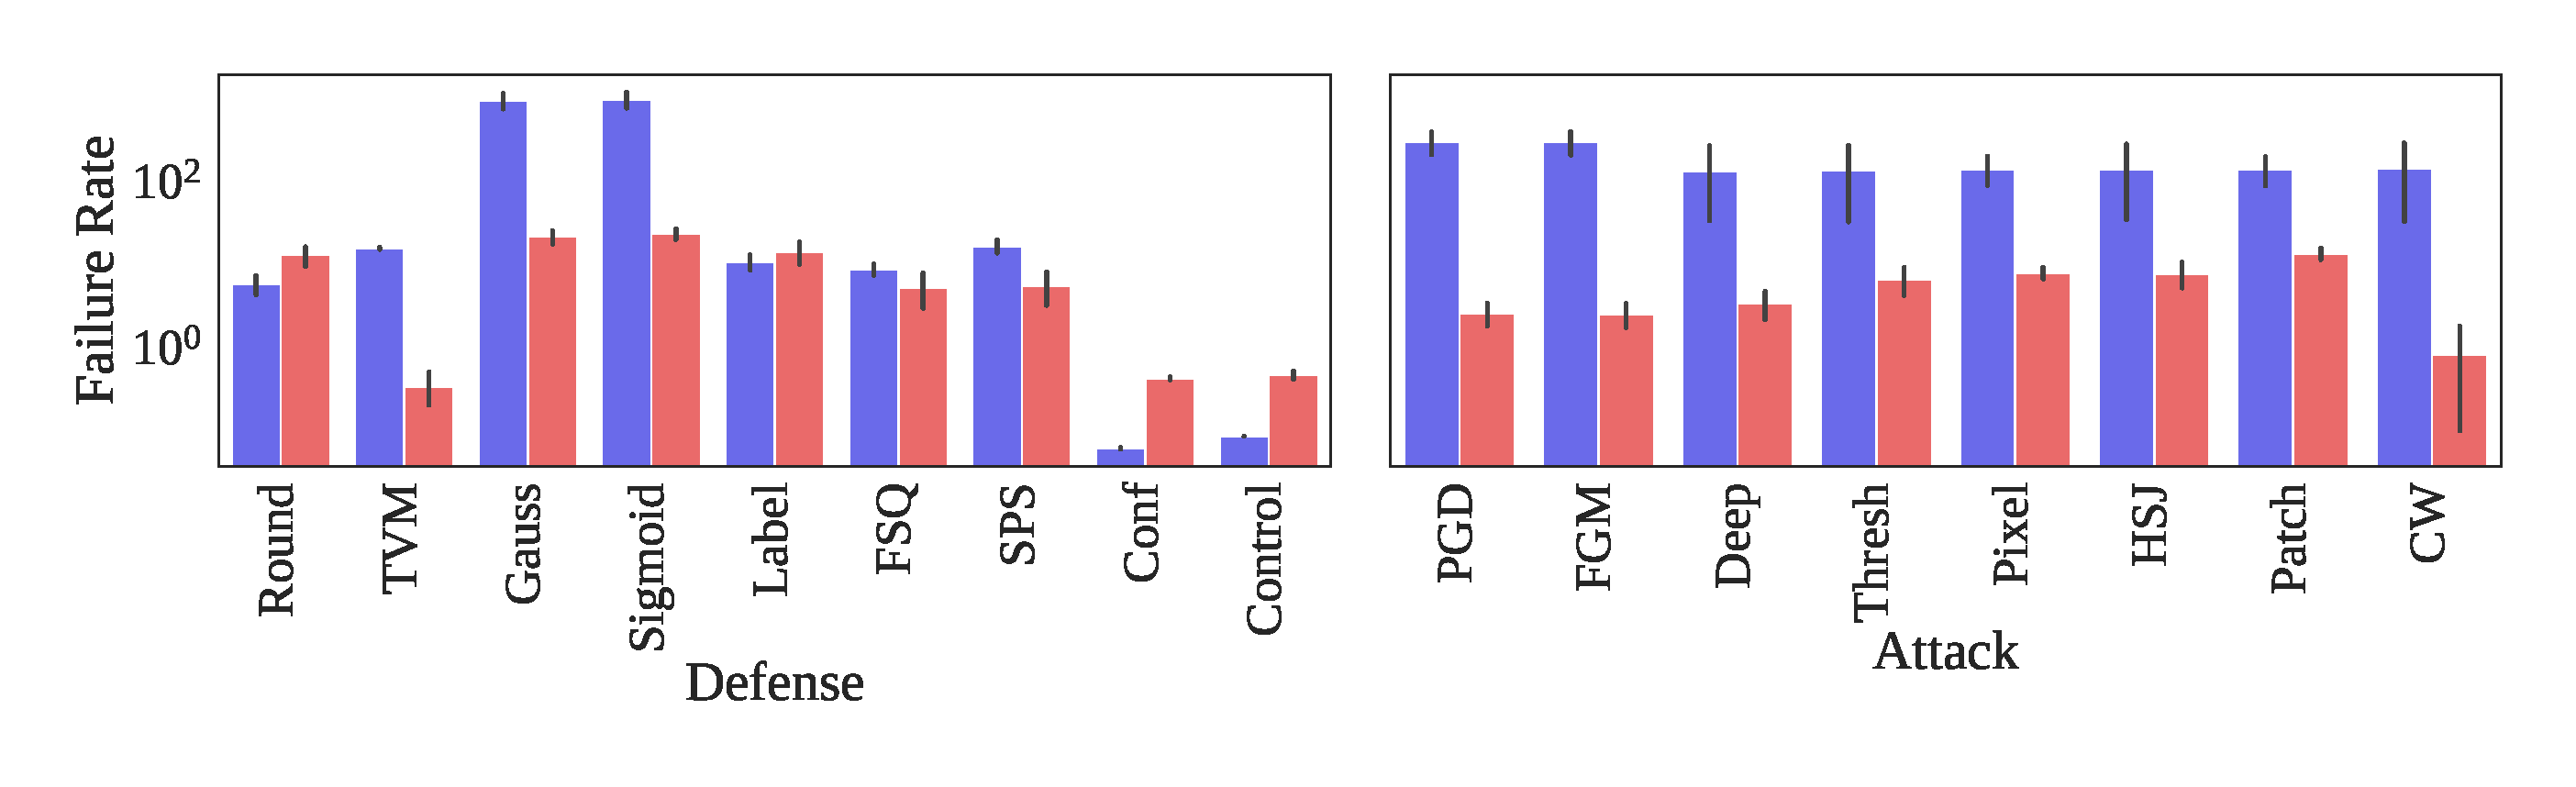
\includegraphics[trim={0 0.85em 0 0.35em},clip,width=0.9\textwidth]{Fig20.eps}
    \vspace{-1em}
    \caption{The 95\% confidence interval of failure rates, both benign (blue) and adversarial (red) on the MNIST dataset, broken down by defense (left) and attack (right). Note that no defense was able to improve upon the benign failure rate. This was computed using Equation~\ref{eq:failure_rate}.}
    \label{fig:mnist_failure_rate}
    } % end centering
\end{figure*}


%% Rate Grid
\begin{figure*}[!hptb]
    {\centering
    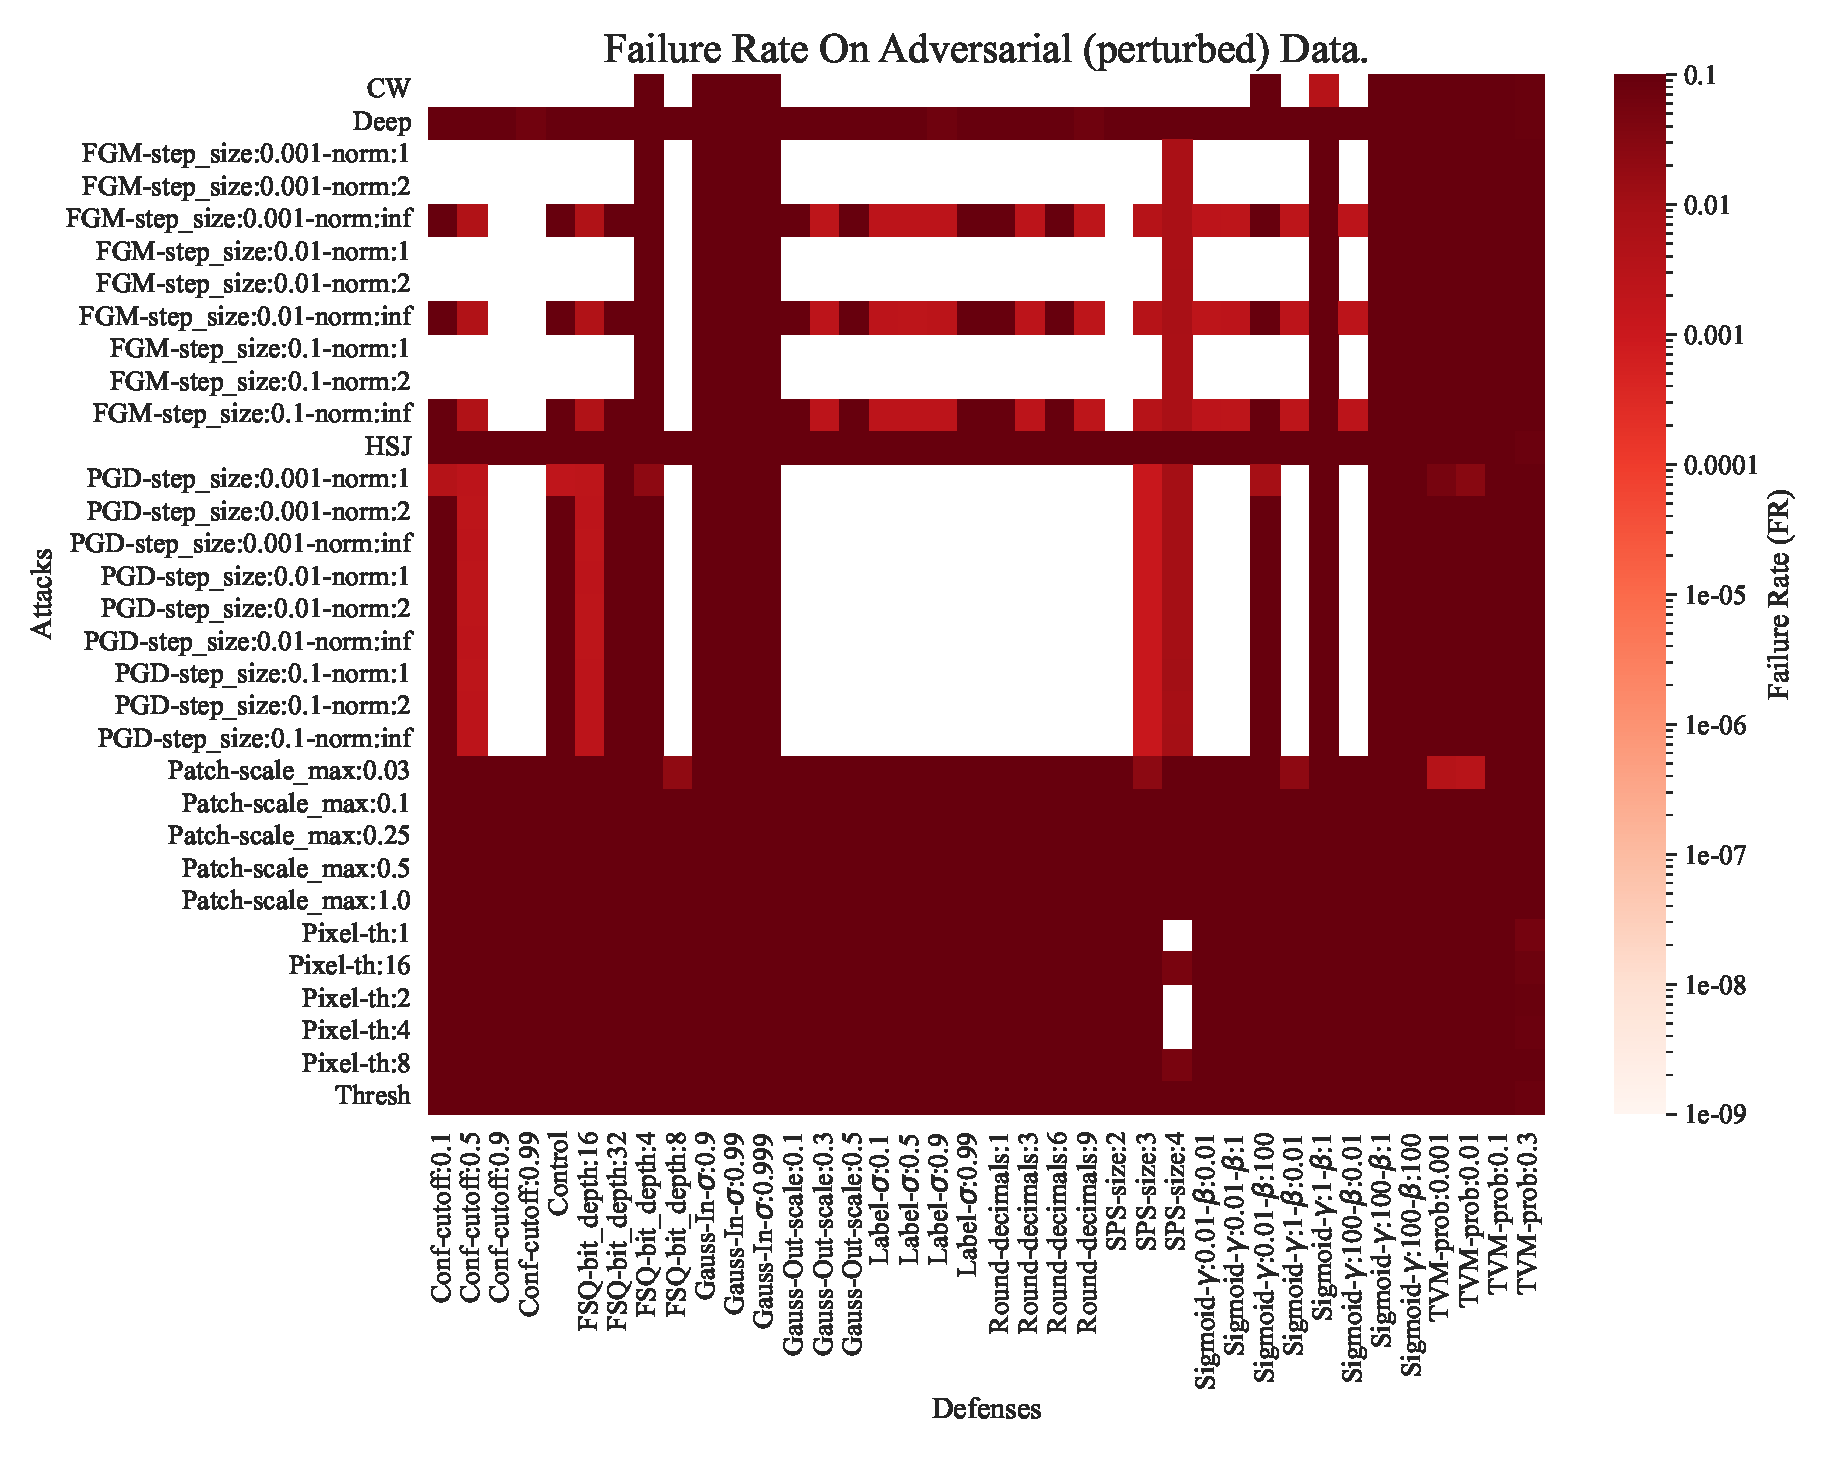
\includegraphics[trim={0 0.85em 0 0.35em},clip,height=0.6\textwidth]{Fig21.eps}
    \vspace{-0.5em}
    \caption{The failure rate for the adversarial case on the MNIST dataset. A darker red indicates a worse performance and white indicates 0 induced failures. Note that the scale is logarithmic so that marginal gains and substantial losses can be seen clearly. White indicates cases where the attack was never successful.}
    \label{fig:mnist_rate_grid}
    } % end centering
\end{figure*}

%% Change Grid
\begin{figure*}[!hptb]
    {\centering
    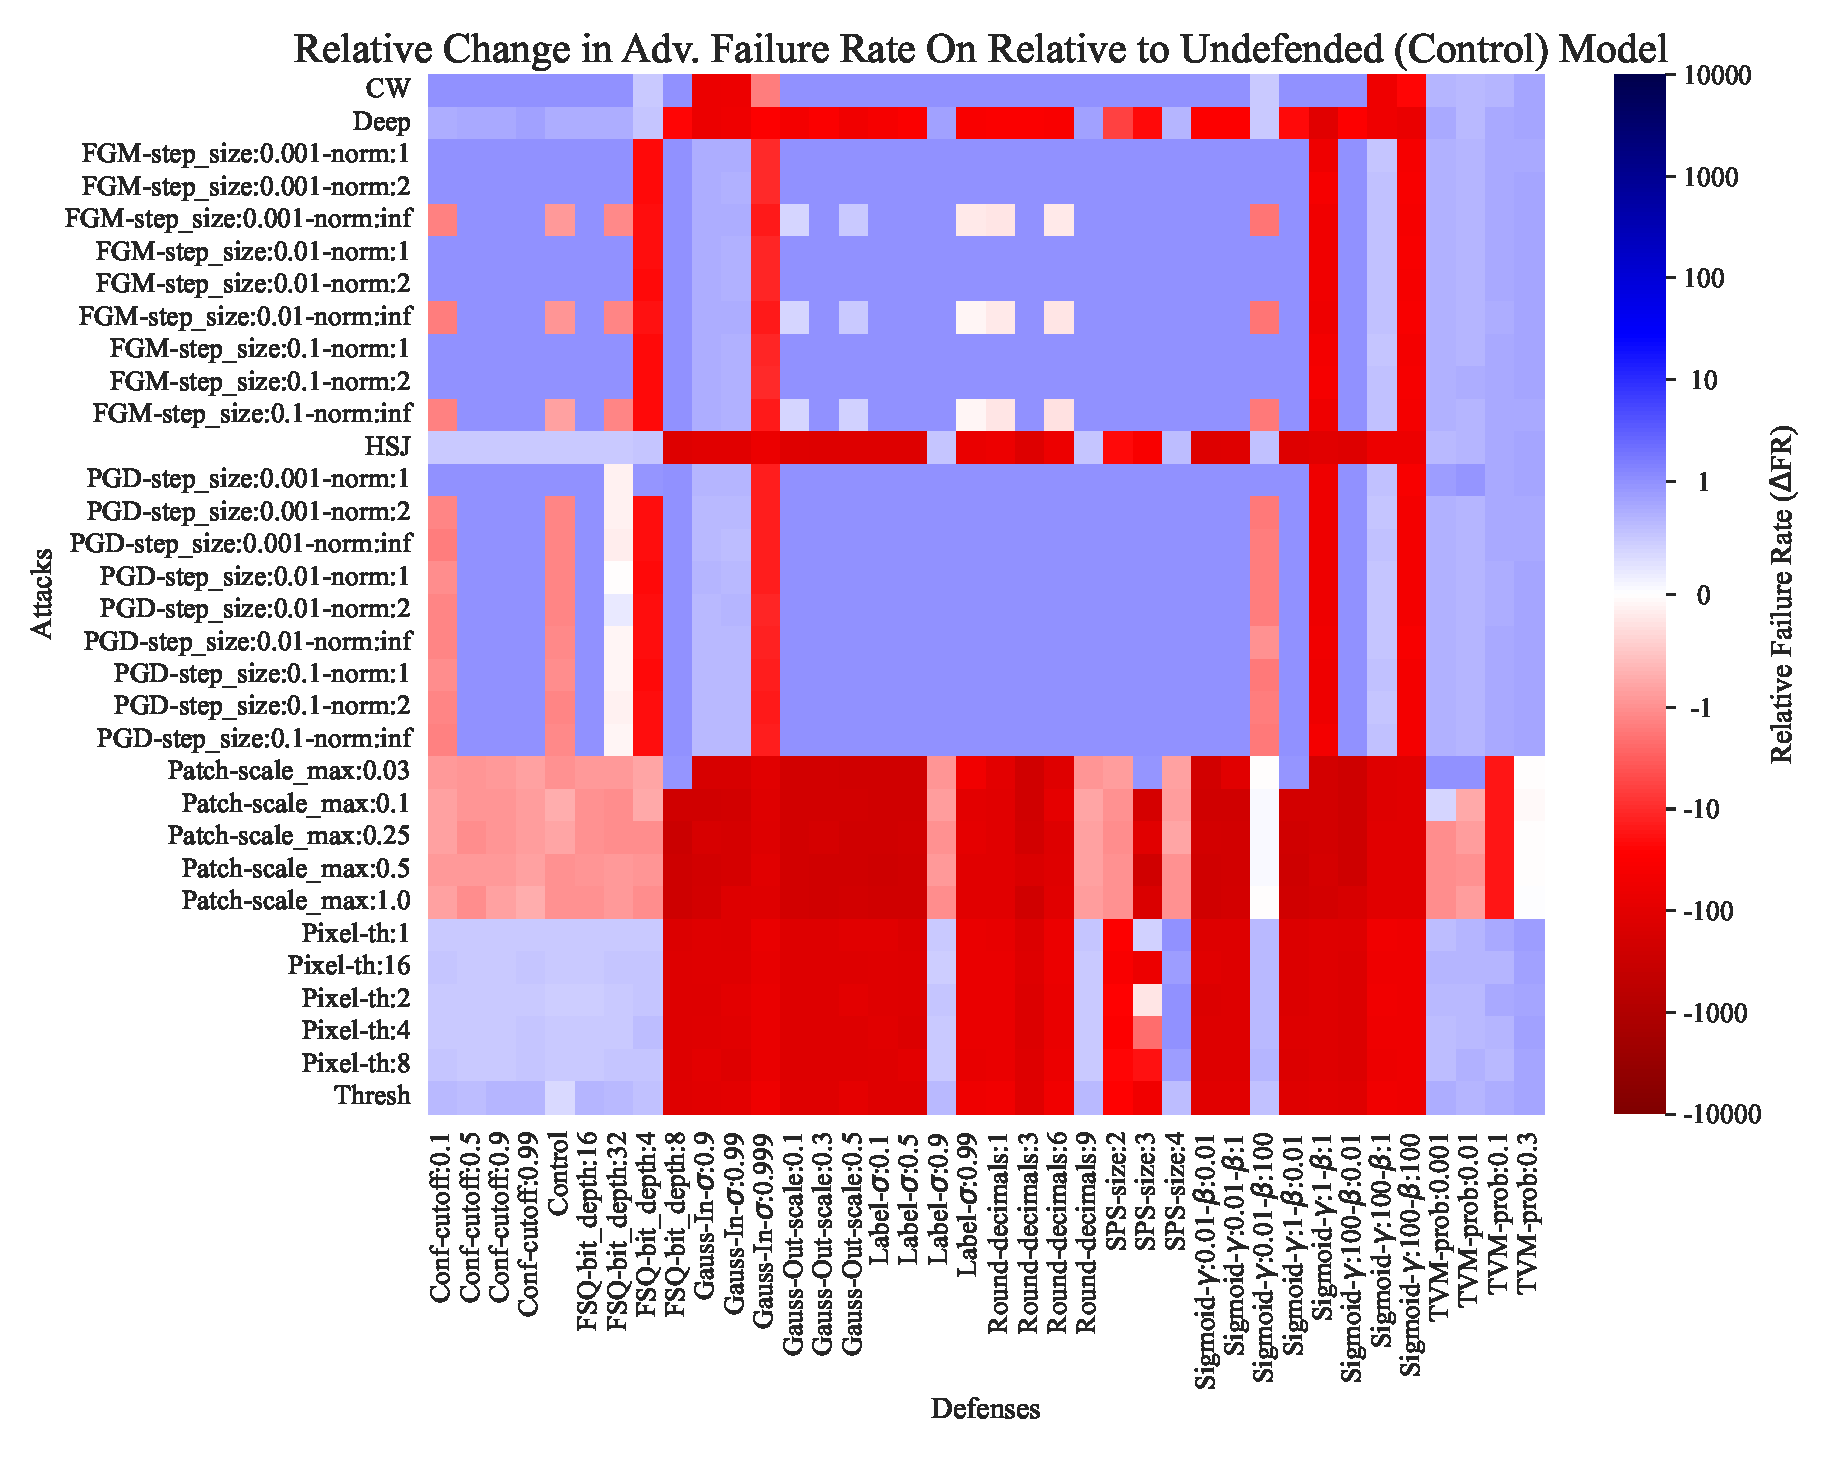
\includegraphics[trim={0 0.85em 0 0.35em},clip,height=0.6\textwidth]{Fig22.eps}
    \vspace{-0.5em}
    \caption{The change in failure rate between the benign and adversarial cases on the MNIST dataset. Blue indicates an improvement relative to the undefended model. Red indicates that defense made a model worse. White indicates no change. Note that the scale is logarithmic so that marginal gains and substantial losses can be seen clearly. This was computed using Equation~\ref{eq:relative_change_failure_rate}.}
    \label{fig:mnist_change_grid}
    } % end centering
\end{figure*}

\section{Limitations}
\cm{[Note: This section has been moved to here. Was previously placed before the results.]}
\label{limitations}
\subsection{True Failure Rate Estimation} 
While it is true that real-world noise can inadvertently become adversarial, it is obvious that not every possible noise vector will increase the loss for a given sample. We can, however, confidently say that the \textit{true generalization error} lies between the test-set accuracy (Eq.~\ref{eq:accuracy}) and the adversarial failure rate. Further work remains regarding the gap between these two estimates, but falls outside the scope of this paper. However, as we show in the results (Section~\ref{results}) this fact hardly matters in the context of modern computer vision models, because \textbf{both of these measures} fail to meet safety-critical standards (see Table~\ref{tab:rate}) by many orders of magnitude (see Fig.~\ref{fig:mnist_failure_rate} and Fig.~\ref{fig:failure_rate}.) 
% So, let $\theta$ be probability that a random feasible (\ie a 1-byte sphere around a given sample) noise vector is adversarial, then chance of failure $\lambda$ at time $t$ is 
% $$
%     \lambda(t|\theta) = \theta \lambda(\theta t).
% $$
% which can be used to approximate the generalized error rate, $\eta$ (Eq.~\ref{eq:accuracy}), using an adversarial estimate of the failure rate (Eq.~\ref{eq:failure_rate}):
% $$
%  \eta \approx \lambda(t | \theta) = \frac{\theta \lambda(\theta t)}{t} =
%      \frac{\mathrm{False~Classifications}}{\mathrm{Total ~Time (s)}},
% $$
% This kind of analysis is quite common in the medical and manufacturing sectors, called `accelerated failure time' modelling~\cite{aft_models} where faster development saves lives and/or reduces time-to-market. 


% Therefore, estimating $\theta$ is out of the scope of this paper. Furthermore, this kind of estimation is, of course, hardware dependent, but would,  nevertheless, be appropriate for product development.}

\subsection{On optimal attacks}
Additionally, while these attacks are quite efficient, none are provably the fastest possible attack. So, \textit{at best}, they \textbf{underestimate} the failure rate. In the case of our safety-critical analysis, this \textbf{amplifies} and \textbf{does not diminish} our claims, raising serious concerns about using in-distribution test data as an indicator of real-world performance. Therefore, because these attacks are not provably optimal, this failure rate should not be taken as an absolute measure of the true failure rate. However, it is still a reliable metric for comparing the efficacy of two models as evidenced by the relatively consistent failure rates across various defenses and hyperparameter configurations for a given attack (right side of Figures~\ref{fig:mnist_failure_rate}~and~\ref{fig:failure_rate}). 
\subsection{Model Selection}
% TODO add several citations from github link
% TODO add eq \labels
In general, we did not choose the model architecture, but relied on two reference models provided by Madry et al. They have been tested and cited numerous times \cite{madry2017towards}. The point of this work is not to chase state-of-the-art results, but to evaluate robustness-maximizing techniques in a controlled manner while highlighting useful metrics and techniques for doing so. At the time of publishing, the authors are not aware of \textit{any} architecture that meets safety critical standards when measured test-set accuracy sense (see~Eq.\ref{eq:accuracy}) and there's no demonstrated technique (to the knowledge of the authors) to reduce this in the adversarial sense without sacrificing accuracy or computational time in the benign case (see~Eq.\ref{eq:failure_rate}, Fig.~\ref{fig:mnist_failure_rate} and Fig.~\ref{fig:failure_rate}). So the general conclusion about the real-time safety-critical nature of modern neural networks would remain the same for any other architecture known to the authors.

\subsection{\cm{On Attacker's Knowledge}}
\cm{In this paper, we have tested white-box attacks (FGM, PGD, CW), attacks that need access to the model probability outputs (Deep, Pixel, Thresh, Patch), and a single black-box method (HSJ), outlined in Sec.~\ref{attacks}. On one hand, it would seemingly be unfair to compare these methods under the same constraints. However, as we show in the results (Sec.~\ref{results}), the apparent advantage of attackers with more knowledge of the model tends to disappear under the added computational burden. That is, the HSJ attack (Sec.~\ref{attacks} and Fig.~\ref{fig:HSJ}), which only relies on hard class-labels and an offline model approximation, is consistently effective at fooling models while also outperforming attacks that have access to more information (see: Figs~\ref{fig:FGM}-~\ref{fig:Patch}). The interesting question, then, isn't necessarily how good of an adversarial sample one can generate, but \textit{the rate} at which \textit{any} misclassification can be induced. This \textit{worst-case failure rate} will define the feasible upper bound on a target hardware architecture. Since these attacks vary substantially in run-time and information requirements, current methods relying on accuracy measures do not distill the efficacy of a given attack or defence from the perspective of any model-builder or attacker with a fixed computational budget. However, by controlling for the number of queries and normalizing by CPU-time (see:~Section~\ref{methods}), we are able to isolate the effect of defence techniques against a wide-variety of idealized attackers that optimize for different distance metrics and are subject to very different constraints. By no means do we want to minimize the offline possibilities (see:~Section~\ref{universal}) of attacks like "Adversarial Patch" and "Hop Skip Jump". Instead, we seek to highlight the \textbf{computational triviality} of these attacks and raise sincere questions about the safety of these models in general.}

\section{Conclusions}

Neural networks are being deployed in a wide variety of industrial applications with real-world safety considerations, that despite high accuracy scores, fail against a wide variety of attacks that overwhelmingly require fewer computational resources than building the original model. While `weak' attacks are fast, they require hyper-parameter tuning and retrospective evaluations that make them less effective, but nonetheless cheap-enough to execute, requiring only a few seconds of CPU time. The efficacy of even single-byte or single-pixel attacks against otherwise very accurate models raises questions not only about the intentional adversary, but also how a system will handle real-world, `legitimate' anomalies like dust, lens aberration, and sensor failure.

When we consider the attack that finds the minimal class-separating distance, DeepFool, we see that 80\% of all samples are corruptible under our meager one-byte distance constraint. When we remove this distance constraint, we find that nearly every sample can be fooled with the addition of an adversarial `patch' on the original image (Figure~\ref{fig:adv_acc_grid}) even when we constrain an attack to a small number of iterations ($\leq 10$). That is, if we assume that our attacker has an unlimited budget, we cannot even hope to defend against these attacks. However, the relative ease of finding such adversarial examples suggests that these attacks provide an empirical estimate of a `worst case' failure rate (see Equation~\ref{eq:failure_rate}) in their respective contexts. Therefore, adversarial model analysis provides a computationally cheap way to analyze the worst case failure rate of a system without having to collect, label, perturb, and predict many thousands of test images.

Furthermore, since this failure rate is based on process time, it is obvious that more powerful hardware, without underlying changes to the model architecture, would result in a larger failure rate since we merely fail on more samples in the same amount of time. That is to say, these problems are inherent to the model and not something that we can solve with more processor cycles. Furthermore, even when we obscure everything from the user except model output, we can consistently break models in as few as ten queries to a hard class-label API (\eg, by using the HopSkipJump attack). We found that adding Gaussian noise to the model outputs or training images, reducing the bit-depth of the numerical calculations to match the precision of the image, and setting a confidence threshold were marginally effective defenses when compared to the control model. However, none of these defenses reach the regulatory standards required for safety-critical systems---in fact, they fail by several orders of magnitude. Furthermore, any gains seen in the failure rate (Figure~\ref{fig:change_grid}) are inconsistent while universally reducing the accuracy on the original (unperturbed/benign) data (Figure~\ref{fig:adv_acc_grid}). Improvements due to the defenses are rare and marginal, and they consistently make benign performance worse (see Figures~\ref{fig:adv_acc_grid} and \ref{fig:mnist_adv_acc_grid}). We find this to be true across both datasets and model architectures. Since we know that model accuracy scales with $\mathcal{O}(1/\sqrt{n})$~\cite{vapnik1994measuring} and attacks seem to run in constant time (see Figures~\ref{fig:time} and \ref{fig:mnist_time}) for a fixed computational and query budgets of a few seconds and 1000 queries respectively. 
% \cm{An additional bound on the minimal attack distance, proven by Dohmatob~\cite{dohmatob_generalized_2019}, demonstrates that marginal gains in the generalized error rate ($\eta$) have an increasingly marginal effect on the volume of the known failure space (for example, a 1-byte sphere around a given sample) since the critical distance scales with $\mathcal{O}(\log(\frac{1}{\eta})$. 
% }
% If we use this better hardware to process more images during training, the accuracy improves as $\mathcal{O}(1/\sqrt{n})$ \cite{vapnik1994measuring} while the costs of such accuracy scale linearly with the number of samples. These extra bits of precision are unlikely to solve the robustness problem as they merely expose more bits to the attacker with each query, which each of the post-processing defenses is designed to minimize anyway. Because adversarial accuracy is tightly coupled to benign accuracy and the ability for a model to generalize (see: Figures~\ref{fig:failure_rate}), improving the benign accuracy seems to penalize the adversarial accuracy by the same degree. That is, more accurate models tend to be more vulnerable to small perturbations of the input since each query reveals more `useful' bits to the attacker. While this can be mitigated somewhat (see: Fig.~\ref{fig:change_grid}), potential gains are marginal and inconsistent.

Finally, due to the rate at which we can generate feasible misclassifications, we must question the real-world efficacy of any system that relies on these models to make predictions that meet the legal standards that define `safe'. Despite this pessimism, adversarial model analysis proves to be a computationally efficient way to analyze and compare the out-of-distribution robustness of model architectures without the need to generate massive test sets from real world data.

\section{Acknowledgements}
Financial support has been provided in part by the Knut and Alice Wallenberg Foundation grant no. 2019.0352 and by the eSSENCE Programme under the Swedish Government’s Strategic Research Initiative.

\FloatBarrier

\bibliographystyle{plain}
\bibliography{bibliography}
\end{document}
